\documentclass[twoside]{book}

% Packages required by doxygen
\usepackage{calc}
\usepackage{doxygen}
\usepackage{graphicx}
\usepackage[utf8]{inputenc}
\usepackage{makeidx}
\usepackage{multicol}
\usepackage{multirow}
\usepackage{textcomp}
\usepackage[table]{xcolor}

% Font selection
\usepackage[T1]{fontenc}
\usepackage{mathptmx}
\usepackage[scaled=.90]{helvet}
\usepackage{courier}
\usepackage{amssymb}
\usepackage{sectsty}
\renewcommand{\familydefault}{\sfdefault}
\allsectionsfont{%
  \fontseries{bc}\selectfont%
  \color{darkgray}%
}
\renewcommand{\DoxyLabelFont}{%
  \fontseries{bc}\selectfont%
  \color{darkgray}%
}

% Page & text layout
\usepackage{geometry}
\geometry{%
  a4paper,%
  top=2.5cm,%
  bottom=2.5cm,%
  left=2.5cm,%
  right=2.5cm%
}
\tolerance=750
\hfuzz=15pt
\hbadness=750
\setlength{\emergencystretch}{15pt}
\setlength{\parindent}{0cm}
\setlength{\parskip}{0.2cm}
\makeatletter
\renewcommand{\paragraph}{%
  \@startsection{paragraph}{4}{0ex}{-1.0ex}{1.0ex}{%
    \normalfont\normalsize\bfseries\SS@parafont%
  }%
}
\renewcommand{\subparagraph}{%
  \@startsection{subparagraph}{5}{0ex}{-1.0ex}{1.0ex}{%
    \normalfont\normalsize\bfseries\SS@subparafont%
  }%
}
\makeatother

% Headers & footers
\usepackage{fancyhdr}
\pagestyle{fancyplain}
\fancyhead[LE]{\fancyplain{}{\bfseries\thepage}}
\fancyhead[CE]{\fancyplain{}{}}
\fancyhead[RE]{\fancyplain{}{\bfseries\leftmark}}
\fancyhead[LO]{\fancyplain{}{\bfseries\rightmark}}
\fancyhead[CO]{\fancyplain{}{}}
\fancyhead[RO]{\fancyplain{}{\bfseries\thepage}}
\fancyfoot[LE]{\fancyplain{}{}}
\fancyfoot[CE]{\fancyplain{}{}}
\fancyfoot[RE]{\fancyplain{}{\bfseries\scriptsize Generated on Thu Dec 17 2015 18\-:57\-:31 for E\-Marche by Doxygen }}
\fancyfoot[LO]{\fancyplain{}{\bfseries\scriptsize Generated on Thu Dec 17 2015 18\-:57\-:31 for E\-Marche by Doxygen }}
\fancyfoot[CO]{\fancyplain{}{}}
\fancyfoot[RO]{\fancyplain{}{}}
\renewcommand{\footrulewidth}{0.4pt}
\renewcommand{\chaptermark}[1]{%
  \markboth{#1}{}%
}
\renewcommand{\sectionmark}[1]{%
  \markright{\thesection\ #1}%
}

% Indices & bibliography
\usepackage{natbib}
\usepackage[titles]{tocloft}
\setcounter{tocdepth}{3}
\setcounter{secnumdepth}{5}
\makeindex

% Custom commands
\newcommand{\clearemptydoublepage}{%
  \newpage{\pagestyle{empty}\cleardoublepage}%
}


%===== C O N T E N T S =====

\begin{document}

% Titlepage & ToC
\pagenumbering{roman}
\begin{titlepage}
\vspace*{7cm}
\begin{center}%
{\Large E\-Marche }\\
\vspace*{1cm}
{\large Generated by Doxygen 1.8.6}\\
\vspace*{0.5cm}
{\small Thu Dec 17 2015 18:57:31}\\
\end{center}
\end{titlepage}
\clearemptydoublepage
\tableofcontents
\clearemptydoublepage
\pagenumbering{arabic}

%--- Begin generated contents ---
\chapter{Hierarchical Index}
\section{Hiérarchie des classes}
Cette liste d'héritage est classée approximativement par ordre alphabétique \-:\begin{DoxyCompactList}
\item \contentsline{section}{Avis}{\pageref{class_avis}}{}
\item \contentsline{section}{Categorie}{\pageref{class_categorie}}{}
\item \contentsline{section}{Coords\-Bancaires}{\pageref{class_coords_bancaires}}{}
\item \contentsline{section}{Etat\-Connexion}{\pageref{class_etat_connexion}}{}
\begin{DoxyCompactList}
\item \contentsline{section}{Etat\-Connecte}{\pageref{class_etat_connecte}}{}
\item \contentsline{section}{Etat\-Deconnecte}{\pageref{class_etat_deconnecte}}{}
\end{DoxyCompactList}
\item \contentsline{section}{Etat\-Vente}{\pageref{class_etat_vente}}{}
\begin{DoxyCompactList}
\item \contentsline{section}{Vente\-Enchere}{\pageref{class_vente_enchere}}{}
\item \contentsline{section}{Vente\-Normale}{\pageref{class_vente_normale}}{}
\end{DoxyCompactList}
\item \contentsline{section}{Gestion\-Bdd}{\pageref{class_gestion_bdd}}{}
\item \contentsline{section}{Les\-Produits}{\pageref{class_les_produits}}{}
\item \contentsline{section}{Les\-Utilisateurs}{\pageref{class_les_utilisateurs}}{}
\item \contentsline{section}{Produit}{\pageref{class_produit}}{}
\item Q\-Dialog\begin{DoxyCompactList}
\item \contentsline{section}{Dialog\-Acheter}{\pageref{class_dialog_acheter}}{}
\item \contentsline{section}{Dialog\-Ajouter\-Vente}{\pageref{class_dialog_ajouter_vente}}{}
\item \contentsline{section}{Dialog\-Connexion}{\pageref{class_dialog_connexion}}{}
\end{DoxyCompactList}
\item Q\-Widget\begin{DoxyCompactList}
\item \contentsline{section}{Ma\-Fenetre}{\pageref{class_ma_fenetre}}{}
\end{DoxyCompactList}
\item \contentsline{section}{Ui\-\_\-\-Dialog\-Acheter}{\pageref{class_ui___dialog_acheter}}{}
\begin{DoxyCompactList}
\item \contentsline{section}{Ui\-:\-:Dialog\-Acheter}{\pageref{class_ui_1_1_dialog_acheter}}{}
\end{DoxyCompactList}
\item \contentsline{section}{Ui\-\_\-\-Dialog\-Ajouter\-Vente}{\pageref{class_ui___dialog_ajouter_vente}}{}
\begin{DoxyCompactList}
\item \contentsline{section}{Ui\-:\-:Dialog\-Ajouter\-Vente}{\pageref{class_ui_1_1_dialog_ajouter_vente}}{}
\end{DoxyCompactList}
\item \contentsline{section}{Ui\-\_\-\-Dialog\-Connexion}{\pageref{class_ui___dialog_connexion}}{}
\begin{DoxyCompactList}
\item \contentsline{section}{Ui\-:\-:Dialog\-Connexion}{\pageref{class_ui_1_1_dialog_connexion}}{}
\end{DoxyCompactList}
\item \contentsline{section}{Ui\-\_\-\-Dialog\-Inscription}{\pageref{class_ui___dialog_inscription}}{}
\begin{DoxyCompactList}
\item \contentsline{section}{Ui\-:\-:Dialog\-Inscription}{\pageref{class_ui_1_1_dialog_inscription}}{}
\end{DoxyCompactList}
\item \contentsline{section}{Ui\-\_\-\-Dialog\-Modification\-Profil}{\pageref{class_ui___dialog_modification_profil}}{}
\begin{DoxyCompactList}
\item \contentsline{section}{Ui\-:\-:Dialog\-Modification\-Profil}{\pageref{class_ui_1_1_dialog_modification_profil}}{}
\end{DoxyCompactList}
\item \contentsline{section}{Utilisateur}{\pageref{class_utilisateur}}{}
\item \contentsline{section}{Vue}{\pageref{class_vue}}{}
\begin{DoxyCompactList}
\item \contentsline{section}{Ma\-Fenetre}{\pageref{class_ma_fenetre}}{}
\end{DoxyCompactList}
\end{DoxyCompactList}

\chapter{Class Index}
\section{Liste des classes}
Liste des classes, structures, unions et interfaces avec une brève description \-:\begin{DoxyCompactList}
\item\contentsline{section}{\hyperlink{class_avis}{Avis} \\*
\begin{DoxyItemize}
\item Représente un avis donné par un utilisateur sur un autre utilisateur ou un produit, avec un commentaire et une note 
\end{DoxyItemize}}{\pageref{class_avis}}{}
\item\contentsline{section}{\hyperlink{class_categorie}{Categorie} \\*
\begin{DoxyItemize}
\item Représente une catégorie de produits 
\end{DoxyItemize}}{\pageref{class_categorie}}{}
\item\contentsline{section}{\hyperlink{class_coords_bancaires}{Coords\-Bancaires} \\*Cette classe contient les données bancaires d'un utilisateur }{\pageref{class_coords_bancaires}}{}
\item\contentsline{section}{\hyperlink{class_dialog_ajouter_vente}{Dialog\-Ajouter\-Vente} \\*
\begin{DoxyItemize}
\item Boîte de dialoque permettant l'ajout d'un produit en vente 
\end{DoxyItemize}}{\pageref{class_dialog_ajouter_vente}}{}
\item\contentsline{section}{\hyperlink{class_dialog_connexion}{Dialog\-Connexion} \\*
\begin{DoxyItemize}
\item Boîte de dialogue permettant de se connecter 
\end{DoxyItemize}}{\pageref{class_dialog_connexion}}{}
\item\contentsline{section}{\hyperlink{class_dialog_inscription}{Dialog\-Inscription} \\*
\begin{DoxyItemize}
\item Boîte de dialogue permettant d'inscrire un nouvel utilisateur 
\end{DoxyItemize}}{\pageref{class_dialog_inscription}}{}
\item\contentsline{section}{\hyperlink{class_dialog_modification_profil}{Dialog\-Modification\-Profil} \\*
\begin{DoxyItemize}
\item Boîte de dialogue permettant de modifier les données du profil utilisateur 
\end{DoxyItemize}}{\pageref{class_dialog_modification_profil}}{}
\item\contentsline{section}{\hyperlink{class_etat_connecte}{Etat\-Connecte} \\*Cette classe gère les utilisateurs connectés }{\pageref{class_etat_connecte}}{}
\item\contentsline{section}{\hyperlink{class_etat_connexion}{Etat\-Connexion} \\*Cette classe gère les états de connexion d'un utilisateur (connecté ou déconnecté) }{\pageref{class_etat_connexion}}{}
\item\contentsline{section}{\hyperlink{class_etat_deconnecte}{Etat\-Deconnecte} \\*Cette classe gère les utilisateurs déconnectés }{\pageref{class_etat_deconnecte}}{}
\item\contentsline{section}{\hyperlink{class_etat_vente}{Etat\-Vente} \\*Cette classe gère l'état d'une vente (enchère ou normale) }{\pageref{class_etat_vente}}{}
\item\contentsline{section}{\hyperlink{class_gestion_bdd}{Gestion\-Bdd} \\*
\begin{DoxyItemize}
\item Gère le stockage des utilisateurs, des produits, et la mise à jour des vues 
\end{DoxyItemize}}{\pageref{class_gestion_bdd}}{}
\item\contentsline{section}{\hyperlink{class_les_produits}{Les\-Produits} \\*Cette classe gère la liste des produits }{\pageref{class_les_produits}}{}
\item\contentsline{section}{\hyperlink{class_les_utilisateurs}{Les\-Utilisateurs} \\*
\begin{DoxyItemize}
\item Gère un vector de pointeurs vers des utilisateurs 
\end{DoxyItemize}}{\pageref{class_les_utilisateurs}}{}
\item\contentsline{section}{\hyperlink{class_ma_fenetre}{Ma\-Fenetre} \\*
\begin{DoxyItemize}
\item Affichage principal de l'application 
\end{DoxyItemize}}{\pageref{class_ma_fenetre}}{}
\item\contentsline{section}{\hyperlink{class_produit}{Produit} \\*Cette classe gère le stockage d'un produit }{\pageref{class_produit}}{}
\item\contentsline{section}{\hyperlink{class_utilisateur}{Utilisateur} \\*
\begin{DoxyItemize}
\item Contient toutes les informations personnelles d'un utilisateur 
\end{DoxyItemize}}{\pageref{class_utilisateur}}{}
\item\contentsline{section}{\hyperlink{class_vente_enchere}{Vente\-Enchere} \\*Cette classe gère une vente aux enchères }{\pageref{class_vente_enchere}}{}
\item\contentsline{section}{\hyperlink{class_vente_normale}{Vente\-Normale} \\*Cette classe gère une vente normale }{\pageref{class_vente_normale}}{}
\item\contentsline{section}{\hyperlink{class_vue}{Vue} \\*
\begin{DoxyItemize}
\item Permet la mise à jour des vues 
\end{DoxyItemize}}{\pageref{class_vue}}{}
\end{DoxyCompactList}

\chapter{Class Documentation}
\section{Dialog\-Ajouter\-Vente Class Reference}
\label{class_dialog_ajouter_vente}\index{Dialog\-Ajouter\-Vente@{Dialog\-Ajouter\-Vente}}
Inheritance diagram for Dialog\-Ajouter\-Vente\-:\begin{figure}[H]
\begin{center}
\leavevmode
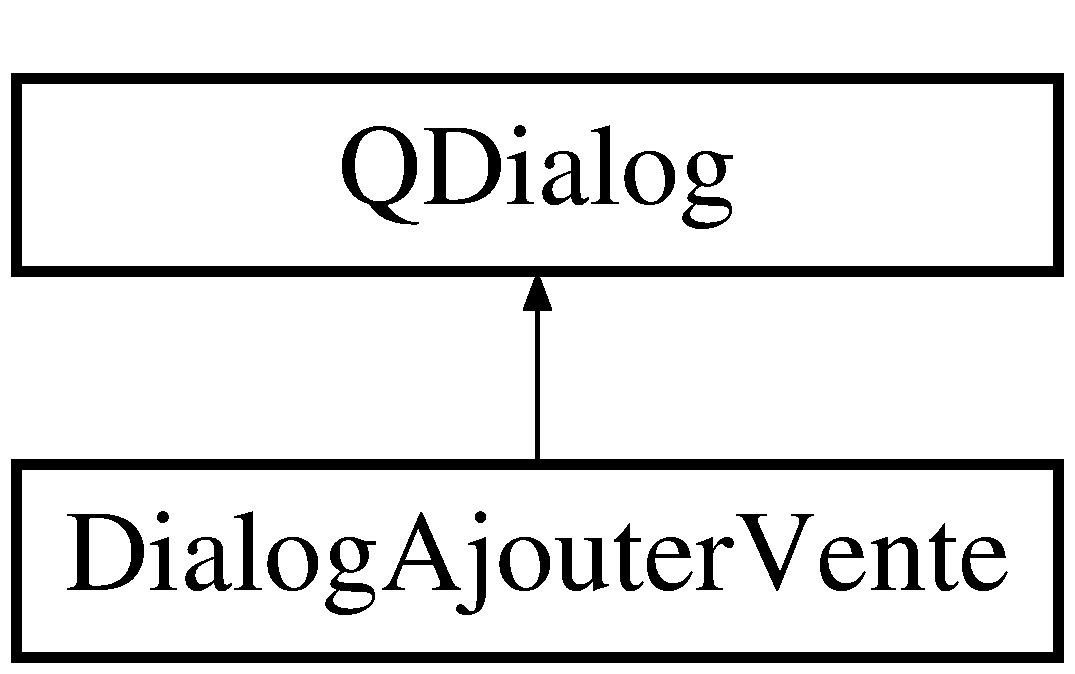
\includegraphics[height=2.000000cm]{class_dialog_ajouter_vente}
\end{center}
\end{figure}
\subsection*{Public Member Functions}
\begin{DoxyCompactItemize}
\item 
{\bfseries Dialog\-Ajouter\-Vente} (Gestion\-Bdd $\ast$bdd, Q\-Widget $\ast$parent=0)\label{class_dialog_ajouter_vente_a891c176f7c824ede407e79dd31b3aafa}

\end{DoxyCompactItemize}


The documentation for this class was generated from the following files\-:\begin{DoxyCompactItemize}
\item 
Dialog\-Ajouter\-Vente.\-h\item 
Dialog\-Ajouter\-Vente.\-cpp\end{DoxyCompactItemize}

\hypertarget{class_ui_1_1_dialog_ajouter_vente}{\section{Référence de la classe Ui\-:\-:Dialog\-Ajouter\-Vente}
\label{class_ui_1_1_dialog_ajouter_vente}\index{Ui\-::\-Dialog\-Ajouter\-Vente@{Ui\-::\-Dialog\-Ajouter\-Vente}}
}


{\ttfamily \#include $<$ui\-\_\-\-Dialog\-Ajouter\-Vente.\-h$>$}

Graphe d'héritage de Ui\-:\-:Dialog\-Ajouter\-Vente\-:\begin{figure}[H]
\begin{center}
\leavevmode
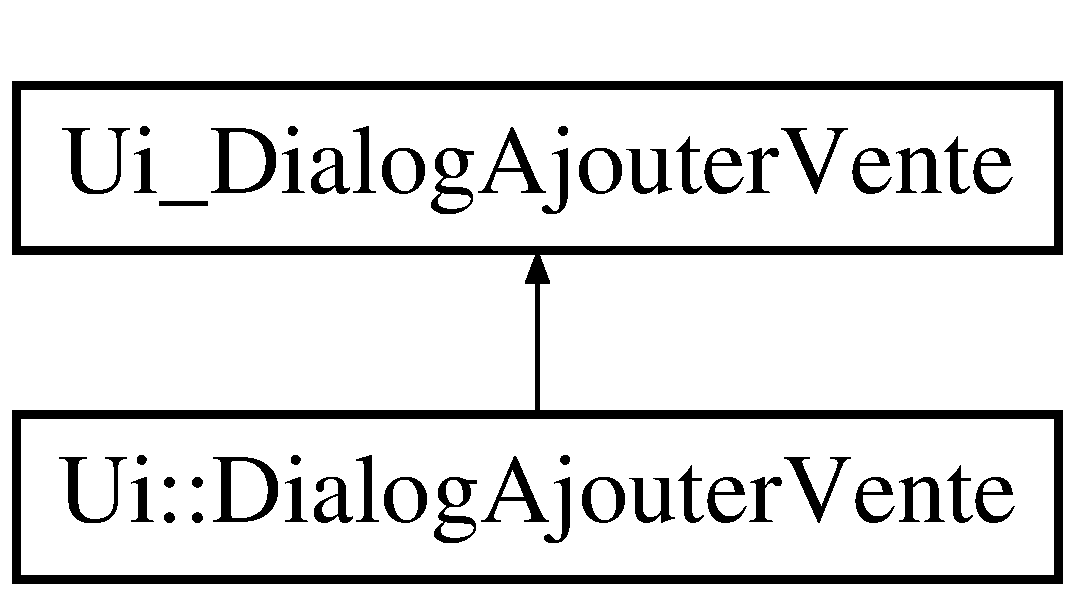
\includegraphics[height=2.000000cm]{class_ui_1_1_dialog_ajouter_vente}
\end{center}
\end{figure}
\subsection*{Membres hérités additionnels}


La documentation de cette classe a été générée à partir du fichier suivant \-:\begin{DoxyCompactItemize}
\item 
/home/magalie/\-Bureau/\-S5/\-C\-P\-O\-O\-A/\-Projet/\-E-\/\-Marche-\//iterations/iteration4/\-E\-Marche/\hyperlink{ui___dialog_ajouter_vente_8h}{ui\-\_\-\-Dialog\-Ajouter\-Vente.\-h}\end{DoxyCompactItemize}

\hypertarget{class_dialog_connexion}{\section{Référence de la classe Dialog\-Connexion}
\label{class_dialog_connexion}\index{Dialog\-Connexion@{Dialog\-Connexion}}
}


The \hyperlink{class_dialog_connexion}{Dialog\-Connexion} class -\/ Boîte de dialogue permettant de se connecter.  




{\ttfamily \#include $<$Dialog\-Connexion.\-h$>$}

Graphe d'héritage de Dialog\-Connexion\-:\begin{figure}[H]
\begin{center}
\leavevmode
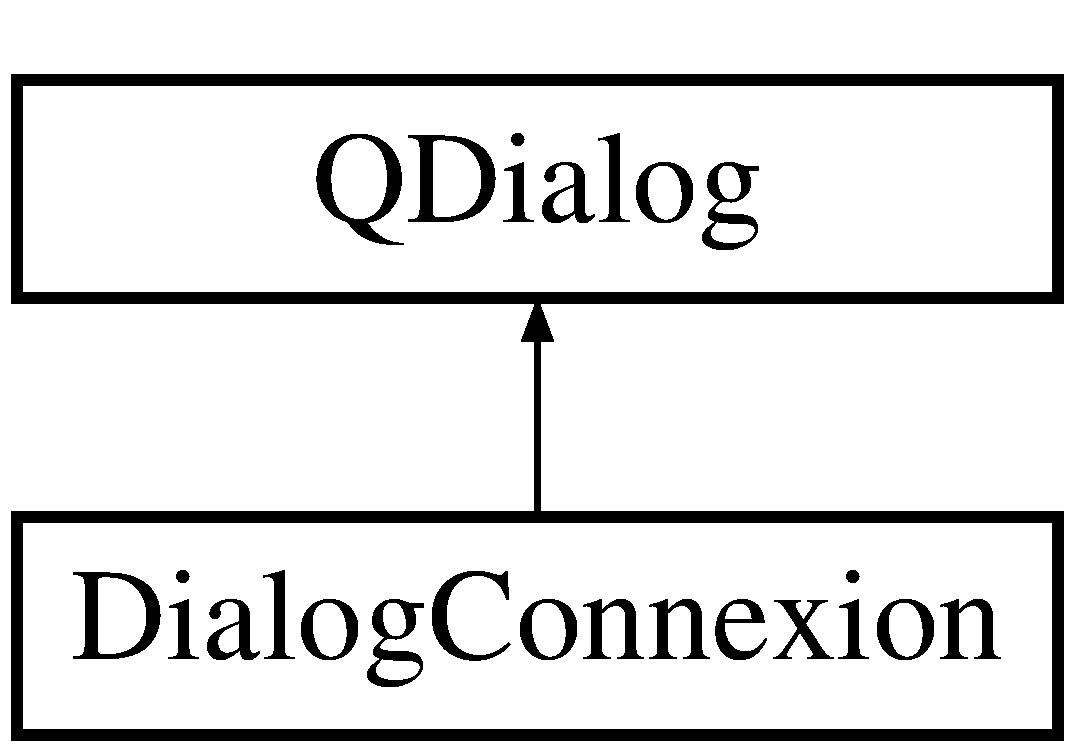
\includegraphics[height=2.000000cm]{class_dialog_connexion}
\end{center}
\end{figure}
\subsection*{Connecteurs publics}
\begin{DoxyCompactItemize}
\item 
void \hyperlink{class_dialog_connexion_aef2d318cc32047ad6c5f7048cc8fb312}{ouvrir} ()
\begin{DoxyCompactList}\small\item\em ouvrir -\/ Affiche la boîte de dialogue \end{DoxyCompactList}\end{DoxyCompactItemize}
\subsection*{Fonctions membres publiques}
\begin{DoxyCompactItemize}
\item 
\hyperlink{class_dialog_connexion_ab104195df6defa3939318919ec495d52}{Dialog\-Connexion} (\hyperlink{class_gestion_bdd}{Gestion\-Bdd} $\ast$bdd, Q\-Widget $\ast$parent=0)
\begin{DoxyCompactList}\small\item\em \hyperlink{class_dialog_connexion}{Dialog\-Connexion} -\/ Constructeur. \end{DoxyCompactList}\item 
\hyperlink{class_dialog_connexion_a1fd101a3631e09a5f87c201960fa61c1}{$\sim$\-Dialog\-Connexion} ()
\end{DoxyCompactItemize}


\subsection{Description détaillée}
The \hyperlink{class_dialog_connexion}{Dialog\-Connexion} class -\/ Boîte de dialogue permettant de se connecter. 

\subsection{Documentation des constructeurs et destructeur}
\hypertarget{class_dialog_connexion_ab104195df6defa3939318919ec495d52}{\index{Dialog\-Connexion@{Dialog\-Connexion}!Dialog\-Connexion@{Dialog\-Connexion}}
\index{Dialog\-Connexion@{Dialog\-Connexion}!DialogConnexion@{Dialog\-Connexion}}
\subsubsection[{Dialog\-Connexion}]{\setlength{\rightskip}{0pt plus 5cm}Dialog\-Connexion\-::\-Dialog\-Connexion (
\begin{DoxyParamCaption}
\item[{{\bf Gestion\-Bdd} $\ast$}]{bdd, }
\item[{Q\-Widget $\ast$}]{parent = {\ttfamily 0}}
\end{DoxyParamCaption}
)\hspace{0.3cm}{\ttfamily [explicit]}}}\label{class_dialog_connexion_ab104195df6defa3939318919ec495d52}


\hyperlink{class_dialog_connexion}{Dialog\-Connexion} -\/ Constructeur. 


\begin{DoxyParams}{Paramètres}
{\em bdd} & -\/ Lien vers \hyperlink{class_gestion_bdd}{Gestion\-Bdd} qui contient toutes les données \\
\hline
{\em parent} & -\/ Lien vers le widget parent \\
\hline
\end{DoxyParams}
\hypertarget{class_dialog_connexion_a1fd101a3631e09a5f87c201960fa61c1}{\index{Dialog\-Connexion@{Dialog\-Connexion}!$\sim$\-Dialog\-Connexion@{$\sim$\-Dialog\-Connexion}}
\index{$\sim$\-Dialog\-Connexion@{$\sim$\-Dialog\-Connexion}!DialogConnexion@{Dialog\-Connexion}}
\subsubsection[{$\sim$\-Dialog\-Connexion}]{\setlength{\rightskip}{0pt plus 5cm}Dialog\-Connexion\-::$\sim$\-Dialog\-Connexion (
\begin{DoxyParamCaption}
{}
\end{DoxyParamCaption}
)}}\label{class_dialog_connexion_a1fd101a3631e09a5f87c201960fa61c1}


\subsection{Documentation des fonctions membres}
\hypertarget{class_dialog_connexion_aef2d318cc32047ad6c5f7048cc8fb312}{\index{Dialog\-Connexion@{Dialog\-Connexion}!ouvrir@{ouvrir}}
\index{ouvrir@{ouvrir}!DialogConnexion@{Dialog\-Connexion}}
\subsubsection[{ouvrir}]{\setlength{\rightskip}{0pt plus 5cm}void Dialog\-Connexion\-::ouvrir (
\begin{DoxyParamCaption}
{}
\end{DoxyParamCaption}
)\hspace{0.3cm}{\ttfamily [slot]}}}\label{class_dialog_connexion_aef2d318cc32047ad6c5f7048cc8fb312}


ouvrir -\/ Affiche la boîte de dialogue 



La documentation de cette classe a été générée à partir des fichiers suivants \-:\begin{DoxyCompactItemize}
\item 
/home/magalie/\-Bureau/\-S5/\-C\-P\-O\-O\-A/\-Projet/\-E-\/\-Marche-\//iterations/iteration2/\-E\-Marche/\hyperlink{_dialog_connexion_8h}{Dialog\-Connexion.\-h}\item 
/home/magalie/\-Bureau/\-S5/\-C\-P\-O\-O\-A/\-Projet/\-E-\/\-Marche-\//iterations/iteration2/\-E\-Marche/\hyperlink{_dialog_connexion_8cpp}{Dialog\-Connexion.\-cpp}\end{DoxyCompactItemize}

\hypertarget{class_ui_1_1_dialog_connexion}{\section{Référence de la classe Ui\-:\-:Dialog\-Connexion}
\label{class_ui_1_1_dialog_connexion}\index{Ui\-::\-Dialog\-Connexion@{Ui\-::\-Dialog\-Connexion}}
}


{\ttfamily \#include $<$ui\-\_\-\-Dialog\-Connexion.\-h$>$}

Graphe d'héritage de Ui\-:\-:Dialog\-Connexion\-:\begin{figure}[H]
\begin{center}
\leavevmode
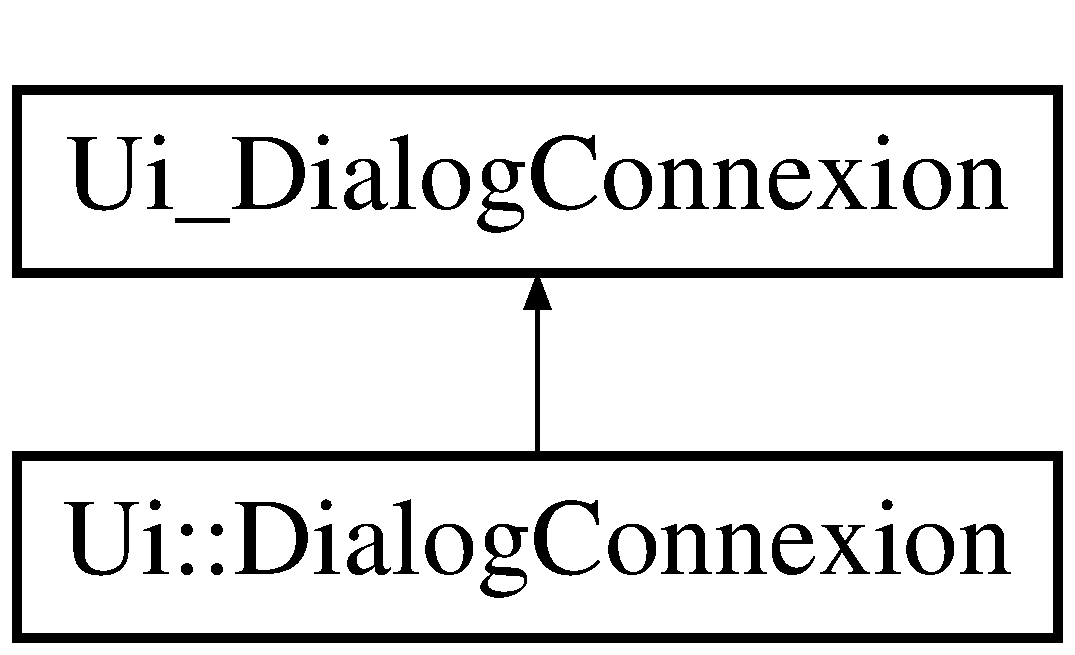
\includegraphics[height=2.000000cm]{class_ui_1_1_dialog_connexion}
\end{center}
\end{figure}
\subsection*{Membres hérités additionnels}


La documentation de cette classe a été générée à partir du fichier suivant \-:\begin{DoxyCompactItemize}
\item 
/home/magalie/\-Bureau/\-S5/\-C\-P\-O\-O\-A/\-Projet/\-E-\/\-Marche-\//iterations/iteration2/\-E\-Marche/\hyperlink{ui___dialog_connexion_8h}{ui\-\_\-\-Dialog\-Connexion.\-h}\end{DoxyCompactItemize}

\hypertarget{class_ui_1_1_dialog_inscription}{\section{Référence de la classe Ui\-:\-:Dialog\-Inscription}
\label{class_ui_1_1_dialog_inscription}\index{Ui\-::\-Dialog\-Inscription@{Ui\-::\-Dialog\-Inscription}}
}


{\ttfamily \#include $<$ui\-\_\-\-Dialog\-Inscription.\-h$>$}

Graphe d'héritage de Ui\-:\-:Dialog\-Inscription\-:\begin{figure}[H]
\begin{center}
\leavevmode
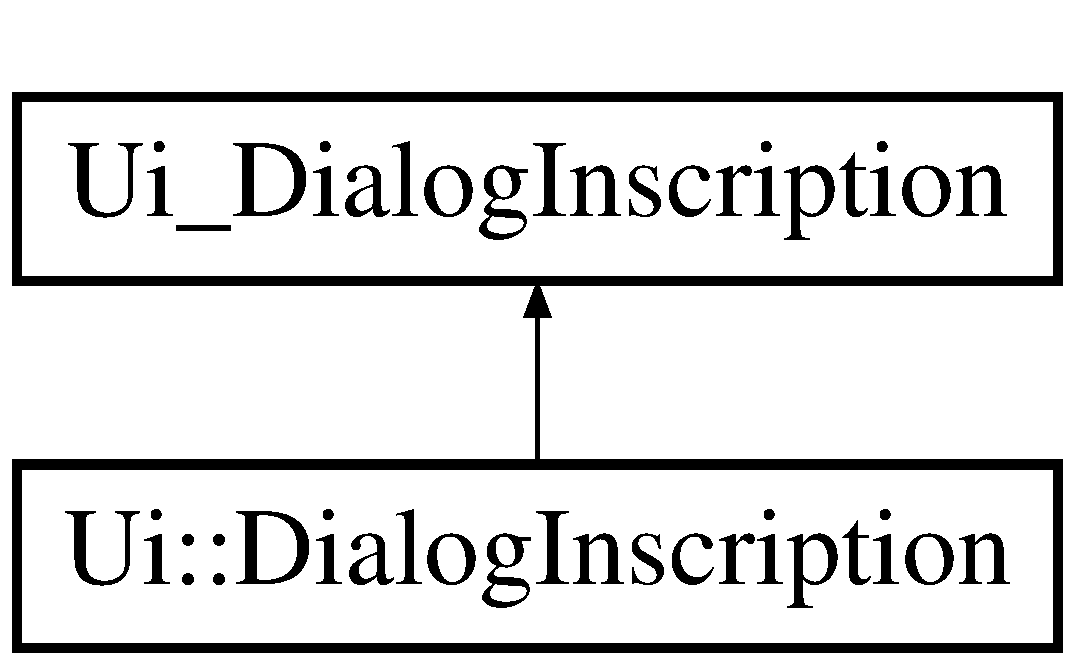
\includegraphics[height=2.000000cm]{class_ui_1_1_dialog_inscription}
\end{center}
\end{figure}
\subsection*{Membres hérités additionnels}


La documentation de cette classe a été générée à partir du fichier suivant \-:\begin{DoxyCompactItemize}
\item 
/home/magalie/\-Bureau/\-S5/\-C\-P\-O\-O\-A/\-Projet/\-E-\/\-Marche-\//iterations/iteration4/\-E\-Marche/\hyperlink{ui___dialog_inscription_8h}{ui\-\_\-\-Dialog\-Inscription.\-h}\end{DoxyCompactItemize}

\hypertarget{class_dialog_inscription}{\section{Référence de la classe Dialog\-Inscription}
\label{class_dialog_inscription}\index{Dialog\-Inscription@{Dialog\-Inscription}}
}


The \hyperlink{class_dialog_inscription}{Dialog\-Inscription} class -\/ Boîte de dialogue permettant d'inscrire un nouvel utilisateur.  




{\ttfamily \#include $<$Dialog\-Inscription.\-h$>$}

Graphe d'héritage de Dialog\-Inscription\-:\begin{figure}[H]
\begin{center}
\leavevmode
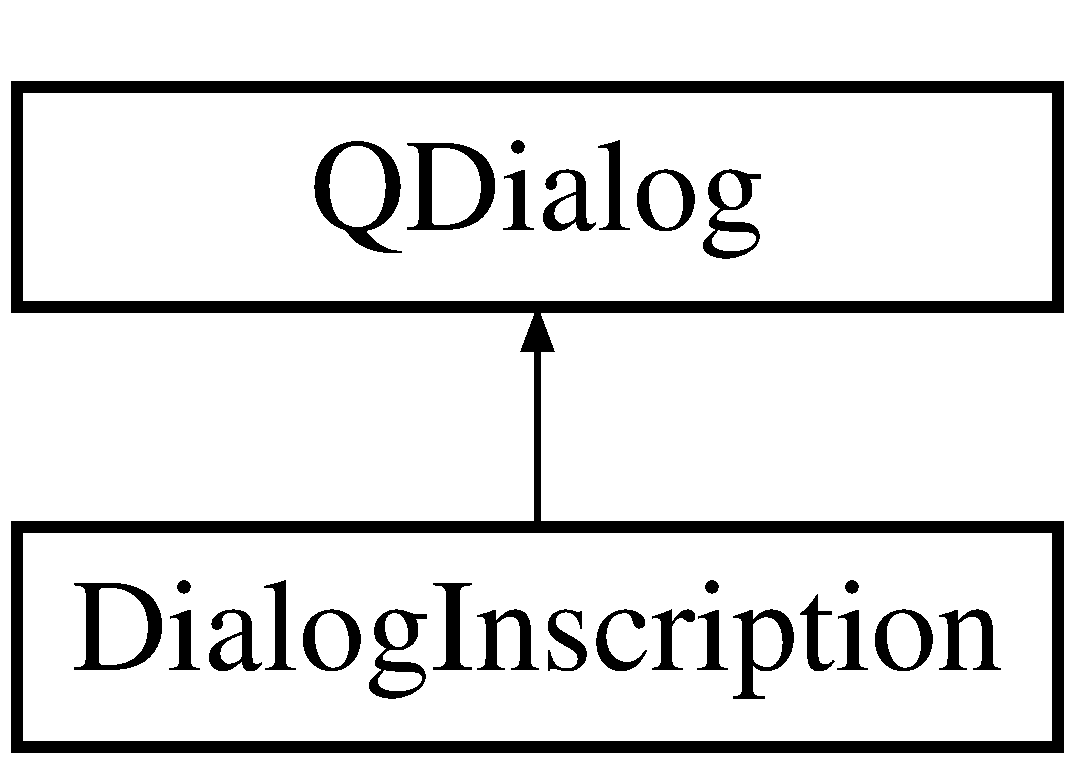
\includegraphics[height=2.000000cm]{class_dialog_inscription}
\end{center}
\end{figure}
\subsection*{Connecteurs publics}
\begin{DoxyCompactItemize}
\item 
void \hyperlink{class_dialog_inscription_ac5daf1277af0ca1e3651f57348ac9169}{ouvrir} ()
\begin{DoxyCompactList}\small\item\em ouvrir -\/ Slot affichant cette boîte de dialogue \end{DoxyCompactList}\end{DoxyCompactItemize}
\subsection*{Fonctions membres publiques}
\begin{DoxyCompactItemize}
\item 
\hyperlink{class_dialog_inscription_ac5cbb6acd3d4f6f9a196a09e99aeb0af}{Dialog\-Inscription} (\hyperlink{class_gestion_bdd}{Gestion\-Bdd} $\ast$bdd, Q\-Widget $\ast$parent=0)
\begin{DoxyCompactList}\small\item\em \hyperlink{class_dialog_inscription}{Dialog\-Inscription} -\/ Constructeur. \end{DoxyCompactList}\item 
\hyperlink{class_dialog_inscription_af6c01135d53fd930ed4f59059fa54563}{$\sim$\-Dialog\-Inscription} ()
\end{DoxyCompactItemize}


\subsection{Description détaillée}
The \hyperlink{class_dialog_inscription}{Dialog\-Inscription} class -\/ Boîte de dialogue permettant d'inscrire un nouvel utilisateur. 

\subsection{Documentation des constructeurs et destructeur}
\hypertarget{class_dialog_inscription_ac5cbb6acd3d4f6f9a196a09e99aeb0af}{\index{Dialog\-Inscription@{Dialog\-Inscription}!Dialog\-Inscription@{Dialog\-Inscription}}
\index{Dialog\-Inscription@{Dialog\-Inscription}!DialogInscription@{Dialog\-Inscription}}
\subsubsection[{Dialog\-Inscription}]{\setlength{\rightskip}{0pt plus 5cm}Dialog\-Inscription\-::\-Dialog\-Inscription (
\begin{DoxyParamCaption}
\item[{{\bf Gestion\-Bdd} $\ast$}]{bdd, }
\item[{Q\-Widget $\ast$}]{parent = {\ttfamily 0}}
\end{DoxyParamCaption}
)\hspace{0.3cm}{\ttfamily [explicit]}}}\label{class_dialog_inscription_ac5cbb6acd3d4f6f9a196a09e99aeb0af}


\hyperlink{class_dialog_inscription}{Dialog\-Inscription} -\/ Constructeur. 


\begin{DoxyParams}{Paramètres}
{\em bdd} & -\/ Lien vers \hyperlink{class_gestion_bdd}{Gestion\-Bdd} qui contient toutes les données \\
\hline
{\em parent} & -\/ Lien vers le widget parent \\
\hline
\end{DoxyParams}
\hypertarget{class_dialog_inscription_af6c01135d53fd930ed4f59059fa54563}{\index{Dialog\-Inscription@{Dialog\-Inscription}!$\sim$\-Dialog\-Inscription@{$\sim$\-Dialog\-Inscription}}
\index{$\sim$\-Dialog\-Inscription@{$\sim$\-Dialog\-Inscription}!DialogInscription@{Dialog\-Inscription}}
\subsubsection[{$\sim$\-Dialog\-Inscription}]{\setlength{\rightskip}{0pt plus 5cm}Dialog\-Inscription\-::$\sim$\-Dialog\-Inscription (
\begin{DoxyParamCaption}
{}
\end{DoxyParamCaption}
)}}\label{class_dialog_inscription_af6c01135d53fd930ed4f59059fa54563}


\subsection{Documentation des fonctions membres}
\hypertarget{class_dialog_inscription_ac5daf1277af0ca1e3651f57348ac9169}{\index{Dialog\-Inscription@{Dialog\-Inscription}!ouvrir@{ouvrir}}
\index{ouvrir@{ouvrir}!DialogInscription@{Dialog\-Inscription}}
\subsubsection[{ouvrir}]{\setlength{\rightskip}{0pt plus 5cm}void Dialog\-Inscription\-::ouvrir (
\begin{DoxyParamCaption}
{}
\end{DoxyParamCaption}
)\hspace{0.3cm}{\ttfamily [slot]}}}\label{class_dialog_inscription_ac5daf1277af0ca1e3651f57348ac9169}


ouvrir -\/ Slot affichant cette boîte de dialogue 



La documentation de cette classe a été générée à partir des fichiers suivants \-:\begin{DoxyCompactItemize}
\item 
/home/magalie/\-Bureau/\-S5/\-C\-P\-O\-O\-A/\-Projet/\-E-\/\-Marche-\//iterations/iteration4/\-E\-Marche/\hyperlink{_dialog_inscription_8h}{Dialog\-Inscription.\-h}\item 
/home/magalie/\-Bureau/\-S5/\-C\-P\-O\-O\-A/\-Projet/\-E-\/\-Marche-\//iterations/iteration4/\-E\-Marche/\hyperlink{_dialog_inscription_8cpp}{Dialog\-Inscription.\-cpp}\end{DoxyCompactItemize}

\hypertarget{class_dialog_modification_profil}{\section{Référence de la classe Dialog\-Modification\-Profil}
\label{class_dialog_modification_profil}\index{Dialog\-Modification\-Profil@{Dialog\-Modification\-Profil}}
}


The \hyperlink{class_dialog_modification_profil}{Dialog\-Modification\-Profil} class -\/ Boîte de dialogue permettant de modifier les données du profil utilisateur.  




{\ttfamily \#include $<$Dialog\-Modification\-Profil.\-h$>$}

Graphe d'héritage de Dialog\-Modification\-Profil\-:\begin{figure}[H]
\begin{center}
\leavevmode
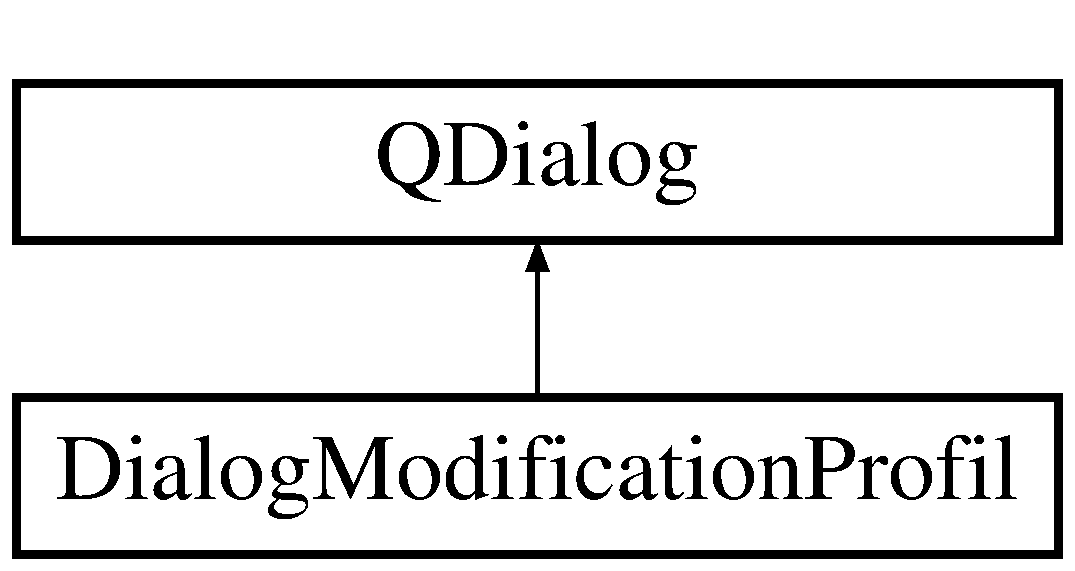
\includegraphics[height=2.000000cm]{class_dialog_modification_profil}
\end{center}
\end{figure}
\subsection*{Fonctions membres publiques}
\begin{DoxyCompactItemize}
\item 
\hyperlink{class_dialog_modification_profil_a700fb3134550ddfa98df89dfca285bb1}{Dialog\-Modification\-Profil} (\hyperlink{class_gestion_bdd}{Gestion\-Bdd} $\ast$bdd, Q\-Widget $\ast$parent=0)
\begin{DoxyCompactList}\small\item\em \hyperlink{class_dialog_modification_profil}{Dialog\-Modification\-Profil} -\/ Constructeur. \end{DoxyCompactList}\item 
\hyperlink{class_dialog_modification_profil_a5f2ede09acd9b01758e4fabe6165e964}{$\sim$\-Dialog\-Modification\-Profil} ()
\end{DoxyCompactItemize}


\subsection{Description détaillée}
The \hyperlink{class_dialog_modification_profil}{Dialog\-Modification\-Profil} class -\/ Boîte de dialogue permettant de modifier les données du profil utilisateur. 

\subsection{Documentation des constructeurs et destructeur}
\hypertarget{class_dialog_modification_profil_a700fb3134550ddfa98df89dfca285bb1}{\index{Dialog\-Modification\-Profil@{Dialog\-Modification\-Profil}!Dialog\-Modification\-Profil@{Dialog\-Modification\-Profil}}
\index{Dialog\-Modification\-Profil@{Dialog\-Modification\-Profil}!DialogModificationProfil@{Dialog\-Modification\-Profil}}
\subsubsection[{Dialog\-Modification\-Profil}]{\setlength{\rightskip}{0pt plus 5cm}Dialog\-Modification\-Profil\-::\-Dialog\-Modification\-Profil (
\begin{DoxyParamCaption}
\item[{{\bf Gestion\-Bdd} $\ast$}]{bdd, }
\item[{Q\-Widget $\ast$}]{parent = {\ttfamily 0}}
\end{DoxyParamCaption}
)\hspace{0.3cm}{\ttfamily [explicit]}}}\label{class_dialog_modification_profil_a700fb3134550ddfa98df89dfca285bb1}


\hyperlink{class_dialog_modification_profil}{Dialog\-Modification\-Profil} -\/ Constructeur. 


\begin{DoxyParams}{Paramètres}
{\em bdd} & -\/ Lien vers \hyperlink{class_gestion_bdd}{Gestion\-Bdd} qui contient toutes les données \\
\hline
{\em parent} & -\/ Lien vers le widget parent \\
\hline
\end{DoxyParams}
\hypertarget{class_dialog_modification_profil_a5f2ede09acd9b01758e4fabe6165e964}{\index{Dialog\-Modification\-Profil@{Dialog\-Modification\-Profil}!$\sim$\-Dialog\-Modification\-Profil@{$\sim$\-Dialog\-Modification\-Profil}}
\index{$\sim$\-Dialog\-Modification\-Profil@{$\sim$\-Dialog\-Modification\-Profil}!DialogModificationProfil@{Dialog\-Modification\-Profil}}
\subsubsection[{$\sim$\-Dialog\-Modification\-Profil}]{\setlength{\rightskip}{0pt plus 5cm}Dialog\-Modification\-Profil\-::$\sim$\-Dialog\-Modification\-Profil (
\begin{DoxyParamCaption}
{}
\end{DoxyParamCaption}
)}}\label{class_dialog_modification_profil_a5f2ede09acd9b01758e4fabe6165e964}


La documentation de cette classe a été générée à partir des fichiers suivants \-:\begin{DoxyCompactItemize}
\item 
\hyperlink{_dialog_modification_profil_8h}{Dialog\-Modification\-Profil.\-h}\item 
\hyperlink{_dialog_modification_profil_8cpp}{Dialog\-Modification\-Profil.\-cpp}\end{DoxyCompactItemize}

\hypertarget{class_ui_1_1_dialog_modification_profil}{\section{Référence de la classe Ui\-:\-:Dialog\-Modification\-Profil}
\label{class_ui_1_1_dialog_modification_profil}\index{Ui\-::\-Dialog\-Modification\-Profil@{Ui\-::\-Dialog\-Modification\-Profil}}
}


{\ttfamily \#include $<$ui\-\_\-\-Dialog\-Modification\-Profil.\-h$>$}

Graphe d'héritage de Ui\-:\-:Dialog\-Modification\-Profil\-:\begin{figure}[H]
\begin{center}
\leavevmode
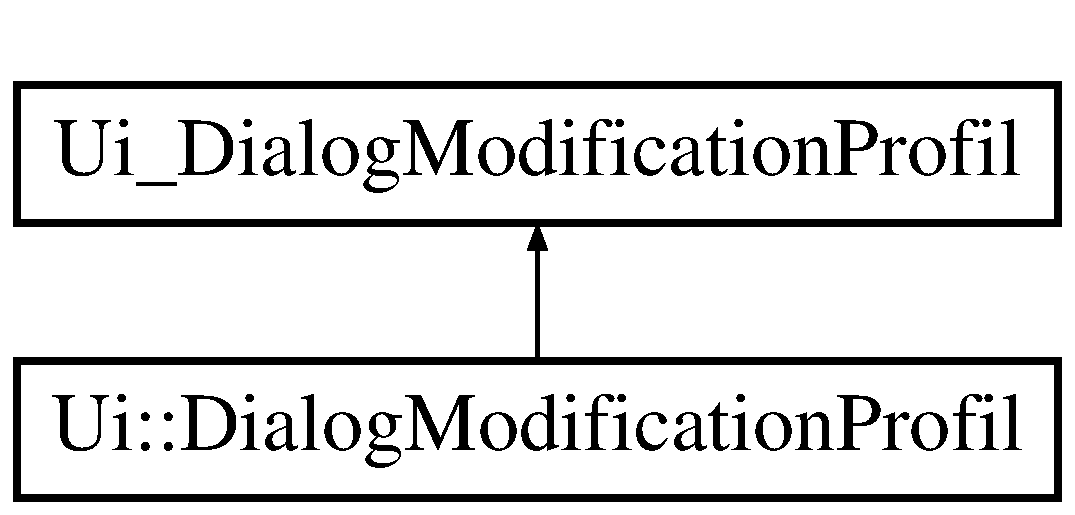
\includegraphics[height=2.000000cm]{class_ui_1_1_dialog_modification_profil}
\end{center}
\end{figure}
\subsection*{Membres hérités additionnels}


La documentation de cette classe a été générée à partir du fichier suivant \-:\begin{DoxyCompactItemize}
\item 
/home/magalie/\-Bureau/\-S5/\-C\-P\-O\-O\-A/\-Projet/\-E-\/\-Marche-\//iterations/iteration2/\-E\-Marche/\hyperlink{ui___dialog_modification_profil_8h}{ui\-\_\-\-Dialog\-Modification\-Profil.\-h}\end{DoxyCompactItemize}

\hypertarget{class_ma_fenetre}{\section{Référence de la classe Ma\-Fenetre}
\label{class_ma_fenetre}\index{Ma\-Fenetre@{Ma\-Fenetre}}
}


The \hyperlink{class_ma_fenetre}{Ma\-Fenetre} class -\/ Affichage principal de l'application.  




{\ttfamily \#include $<$Ma\-Fenetre.\-h$>$}

Graphe d'héritage de Ma\-Fenetre\-:\begin{figure}[H]
\begin{center}
\leavevmode
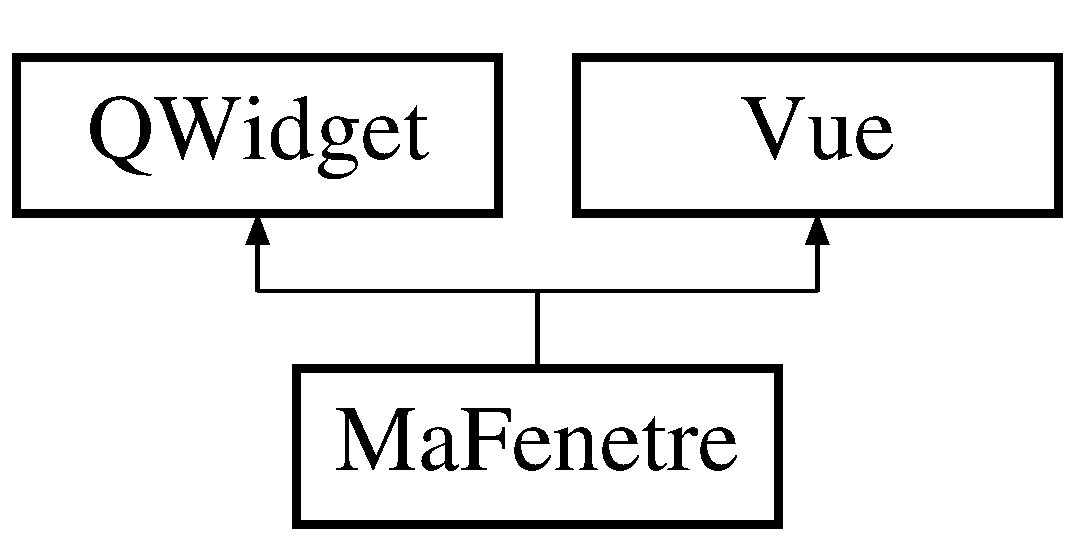
\includegraphics[height=2.000000cm]{class_ma_fenetre}
\end{center}
\end{figure}
\subsection*{Connecteurs publics}
\begin{DoxyCompactItemize}
\item 
void \hyperlink{class_ma_fenetre_a115348adbe409a24a0d381e1fcc62fe7}{afficher\-Res\-Produits} (std\-::vector$<$ \hyperlink{class_produit}{Produit} $\ast$ $>$ v)
\begin{DoxyCompactList}\small\item\em afficher\-Res\-Produits -\/ Affiche le résultat d'une recherche de produit \end{DoxyCompactList}\item 
void \hyperlink{class_ma_fenetre_a8107c2666807db431962fdcd4e942c69}{rechercher} ()
\begin{DoxyCompactList}\small\item\em rechercher -\/ Redirige vers l'affichage d'utilisateurs ou de produits selon le type de recherche lancé \end{DoxyCompactList}\item 
void \hyperlink{class_ma_fenetre_abc0a097122f161ced271718b254206cd}{accueil} ()
\begin{DoxyCompactList}\small\item\em accueil -\/ Affiche les produits en vente actuellement \end{DoxyCompactList}\item 
void \hyperlink{class_ma_fenetre_a08a81ac61e783cf5ed3855ca4f18c84e}{profil} ()
\begin{DoxyCompactList}\small\item\em profil -\/ Affiche le profil de l'utilisateur connecté \end{DoxyCompactList}\item 
void \hyperlink{class_ma_fenetre_abdebcc3a608ba960f92d9c33198afa8e}{statistiques} ()
\begin{DoxyCompactList}\small\item\em statistiques -\/ Affiche les statistiques de l'utilisateur connecté \end{DoxyCompactList}\item 
void \hyperlink{class_ma_fenetre_ae0699859505bac920f9cb033ddb1da23}{ventes} ()
\begin{DoxyCompactList}\small\item\em ventes -\/ Affiche les ventes de l'utilisateur connecté \end{DoxyCompactList}\item 
void \hyperlink{class_ma_fenetre_a48f619e7d913b0e969273be7435b9ab5}{achats} ()
\begin{DoxyCompactList}\small\item\em achats -\/ Affiche les achats de l'utilisateur connecté \end{DoxyCompactList}\item 
void \hyperlink{class_ma_fenetre_abd8cb1d6b536873f3d369457073270c4}{ajouter\-Vente} ()
\begin{DoxyCompactList}\small\item\em ajouter\-Vente -\/ Ouvre la boîte de dialogue permettant d'ajouter une vente si on est connecté \end{DoxyCompactList}\item 
void \hyperlink{class_ma_fenetre_a65270bfc0eeecb1003c6abc9a1199f32}{connexion} ()
\begin{DoxyCompactList}\small\item\em connexion -\/ Ouvre la boîte de dialogue de connexion \end{DoxyCompactList}\item 
void \hyperlink{class_ma_fenetre_a4568c5e0376f04b9d1ab6c54b9f7c7ed}{modification\-Profil} ()
\begin{DoxyCompactList}\small\item\em modification\-Profil -\/ Ouvre la boîte de dialogue de modification de profil de l'utilisateur connecté \end{DoxyCompactList}\item 
void \hyperlink{class_ma_fenetre_ade3a46e2b308936d934503a88275495a}{voir\-Produit} (Q\-String ref)
\begin{DoxyCompactList}\small\item\em voir\-Produit -\/ Affiche les données du produit et permet de l'acheter \end{DoxyCompactList}\item 
void \hyperlink{class_ma_fenetre_a44eae809341ad4816d8ca151d9b703fb}{acheter} ()
\begin{DoxyCompactList}\small\item\em acheter -\/ Achète le produit si on est connecté \end{DoxyCompactList}\end{DoxyCompactItemize}
\subsection*{Signaux}
\begin{DoxyCompactItemize}
\item 
void \hyperlink{class_ma_fenetre_a75cd895beb38fe68a4319eb6c37ac8ee}{signal\-Recherche\-Produits} (std\-::vector$<$ \hyperlink{class_produit}{Produit} $\ast$ $>$ v)
\begin{DoxyCompactList}\small\item\em signal\-Recherche\-Produits -\/ Signale qu'il s'agit d'une recherche de produits \end{DoxyCompactList}\end{DoxyCompactItemize}
\subsection*{Fonctions membres publiques}
\begin{DoxyCompactItemize}
\item 
\hyperlink{class_ma_fenetre_ae39212ca7a4d4b4c99a13b1d5eb063fa}{Ma\-Fenetre} (int l, int h, \hyperlink{class_gestion_bdd}{Gestion\-Bdd} $\ast$bdd)
\begin{DoxyCompactList}\small\item\em \hyperlink{class_ma_fenetre}{Ma\-Fenetre} -\/ Constructeur. \end{DoxyCompactList}\item 
\hyperlink{class_ma_fenetre_a2396ba2918e49df8d0c4a8c70f927151}{$\sim$\-Ma\-Fenetre} ()
\item 
void \hyperlink{class_ma_fenetre_a342da912af9b611d47229fd190d68522}{update} ()
\begin{DoxyCompactList}\small\item\em update -\/ Mets à jour la fenêtre principal \end{DoxyCompactList}\item 
void \hyperlink{class_ma_fenetre_a4bc520a56473760bb8433a1de67da378}{clear\-Layout} (Q\-Layout $\ast$layout)
\begin{DoxyCompactList}\small\item\em clear\-Layout -\/ Vide un layout entré en paramètre \end{DoxyCompactList}\end{DoxyCompactItemize}
\subsection*{Attributs protégés}
\begin{DoxyCompactItemize}
\item 
Q\-H\-Box\-Layout $\ast$ \hyperlink{class_ma_fenetre_acd485d3f85c155925df773f028f9e537}{haut}
\begin{DoxyCompactList}\small\item\em haut -\/ Contient la barre de recherche, l'accueil, l'ajout de vente, mon profil, connexion \end{DoxyCompactList}\item 
Q\-V\-Box\-Layout $\ast$ \hyperlink{class_ma_fenetre_aefa40adcb6099816353c31ea230ec1af}{centre}
\begin{DoxyCompactList}\small\item\em centre -\/ Contient le titre de ce qu'on affiche au centre et les affichages \end{DoxyCompactList}\item 
Q\-H\-Box\-Layout $\ast$ \hyperlink{class_ma_fenetre_a6e267fbdcd8da190e956c593664587c6}{centre\-Profil}
\begin{DoxyCompactList}\small\item\em centre\-Profil -\/ Contient l'affichage du profil \end{DoxyCompactList}\item 
Q\-H\-Box\-Layout $\ast$ \hyperlink{class_ma_fenetre_aff3315e53711db117feadab319660cee}{bas}
\begin{DoxyCompactList}\small\item\em bas -\/ Contient le changement de pages \end{DoxyCompactList}\item 
Q\-Combo\-Box $\ast$ \hyperlink{class_ma_fenetre_a3df6a320b8835369da88bf94b701ae76}{type\-Recherche}
\begin{DoxyCompactList}\small\item\em type\-Recherche -\/ Type de la recherche \-: \hyperlink{class_produit}{Produit} ou \hyperlink{class_utilisateur}{Utilisateur} \end{DoxyCompactList}\item 
Q\-Line\-Edit $\ast$ \hyperlink{class_ma_fenetre_a37836681a6d48a32dcd379b11447f579}{val\-Recherche}
\begin{DoxyCompactList}\small\item\em val\-Recherche -\/ Ce que l'on veut rechercher \end{DoxyCompactList}\item 
Q\-Push\-Button $\ast$ \hyperlink{class_ma_fenetre_afe6e47d40e487fccd18d4bcc3c57e64e}{bouton\-Recherche}
\begin{DoxyCompactList}\small\item\em bouton\-Recherche -\/ Lancement de la recherche \end{DoxyCompactList}\item 
Q\-Push\-Button $\ast$ \hyperlink{class_ma_fenetre_a0316aa06b89b812a8528a8ccbe81561a}{bouton\-Accueil}
\begin{DoxyCompactList}\small\item\em bouton\-Accueil -\/ Affichage des ventes en cours \end{DoxyCompactList}\item 
Q\-Push\-Button $\ast$ \hyperlink{class_ma_fenetre_a406ca1016af97e007bc633efabed744b}{bouton\-Profil}
\begin{DoxyCompactList}\small\item\em bouton\-Profil -\/ Affichage du profil de l'utilisateur \end{DoxyCompactList}\item 
Q\-Push\-Button $\ast$ \hyperlink{class_ma_fenetre_a422d1e619aa51ff42b5ecd2c5476ce19}{bouton\-Ajouter\-Vente}
\begin{DoxyCompactList}\small\item\em bouton\-Ajouter\-Vente -\/ Permet d'ajouter un produit en vente \end{DoxyCompactList}\item 
Q\-Push\-Button $\ast$ \hyperlink{class_ma_fenetre_ac438e7ad115265305422aadd11a04b50}{bouton\-Statistiques}
\begin{DoxyCompactList}\small\item\em bouton\-Statistiques -\/ Affichage des statistiques utilisateur \end{DoxyCompactList}\item 
Q\-Push\-Button $\ast$ \hyperlink{class_ma_fenetre_a9399bb35a8e0a832597a2f3cb4e8dea3}{bouton\-Ventes}
\begin{DoxyCompactList}\small\item\em bouton\-Ventes -\/ Affichage des ventes utilisateur \end{DoxyCompactList}\item 
Q\-Push\-Button $\ast$ \hyperlink{class_ma_fenetre_aba39f3cf91351a7d6d0a6188ac831ad5}{bouton\-Achats}
\begin{DoxyCompactList}\small\item\em bouton\-Achats -\/ Affichage des achats utilisateurs \end{DoxyCompactList}\item 
Q\-Push\-Button $\ast$ \hyperlink{class_ma_fenetre_abfdb548dc88cf56eae01fd20be7b052a}{bouton\-Compte}
\begin{DoxyCompactList}\small\item\em bouton\-Compte -\/ Affichage du profil de l'utilisateur connecté \end{DoxyCompactList}\item 
Q\-Label $\ast$ \hyperlink{class_ma_fenetre_ae7932944c172401e793af721335e7c3d}{pseudo\-Connecte}
\begin{DoxyCompactList}\small\item\em pseudo\-Connecte -\/ Affichage du pseudo de l'utilisateur connecté \end{DoxyCompactList}\item 
Q\-Push\-Button $\ast$ \hyperlink{class_ma_fenetre_a6654bb6885a843d1a6ad9399eb7d0c36}{bouton\-Connexion}
\begin{DoxyCompactList}\small\item\em bouton\-Connexion -\/ Permet de se connecter/déconnecter \end{DoxyCompactList}\item 
Q\-Label $\ast$ \hyperlink{class_ma_fenetre_ac4749f9608f7c8d6e5d60434ddbedfc5}{titre\-Section}
\begin{DoxyCompactList}\small\item\em titre\-Section -\/ Affiche le titre de ce qu'on affiche au centre \end{DoxyCompactList}\item 
Q\-Scroll\-Area $\ast$ \hyperlink{class_ma_fenetre_a4f199f65ae682c48c837875a486d2f3f}{barre\-Defile}
\begin{DoxyCompactList}\small\item\em barre\-Defile -\/ \char`\"{}\-Cadre\char`\"{} du centre de l'affichage \end{DoxyCompactList}\item 
Q\-Push\-Button $\ast$ \hyperlink{class_ma_fenetre_a53b01801ba121b8240df4f1f8c9330b3}{bouton\-Precedent}
\begin{DoxyCompactList}\small\item\em bouton\-Precedent -\/ Permet de passer à la page précédente \end{DoxyCompactList}\item 
Q\-Push\-Button $\ast$ \hyperlink{class_ma_fenetre_a54110f455a71febc15224b68470dd80e}{bouton\-Suivant}
\begin{DoxyCompactList}\small\item\em bouton\-Suivant -\/ Permet de passer à la page suivante \end{DoxyCompactList}\item 
Q\-Label $\ast$ \hyperlink{class_ma_fenetre_a941eff753d1e20d0ef212aa875570330}{num\-Page}
\begin{DoxyCompactList}\small\item\em num\-Page -\/ Affiche le numéro de page actuel \end{DoxyCompactList}\item 
\hyperlink{class_dialog_modification_profil}{Dialog\-Modification\-Profil} $\ast$ \hyperlink{class_ma_fenetre_accfaae414323cd476f255f51a98414f0}{modif\-Profil}
\begin{DoxyCompactList}\small\item\em modif\-Profil -\/ Boîte de dilaogue de modification de profil \end{DoxyCompactList}\item 
\hyperlink{class_dialog_ajouter_vente}{Dialog\-Ajouter\-Vente} $\ast$ \hyperlink{class_ma_fenetre_a2332279c45b76ac1c9daf739c0bb3958}{ajouter\-Ventes}
\begin{DoxyCompactList}\small\item\em ajouter\-Ventes -\/ Boîte de dialogue d'ajout de vente \end{DoxyCompactList}\item 
\hyperlink{class_dialog_connexion}{Dialog\-Connexion} $\ast$ \hyperlink{class_ma_fenetre_a3c115601ad85a01422813dcdf48eb44d}{connexions}
\begin{DoxyCompactList}\small\item\em connexions -\/ Boîte de dialogue de connexion \end{DoxyCompactList}\item 
\hyperlink{class_dialog_acheter}{Dialog\-Acheter} $\ast$ \hyperlink{class_ma_fenetre_a8682e6343da2d0c2bfe1fab3ff0e7baa}{acheter\-Quantite}
\begin{DoxyCompactList}\small\item\em achats -\/ Boîte de dialogue d'achats \end{DoxyCompactList}\item 
int \hyperlink{class_ma_fenetre_abe37db89fd8895cc34ccc0f5cda67aaf}{largeur}
\begin{DoxyCompactList}\small\item\em largeur -\/ largeur de la fenêtre \end{DoxyCompactList}\item 
int \hyperlink{class_ma_fenetre_ae1a802d46705239d08d3bf06cd99b802}{hauteur}
\begin{DoxyCompactList}\small\item\em hauteur -\/ hauteur de la fenêtre \end{DoxyCompactList}\item 
\hyperlink{class_gestion_bdd}{Gestion\-Bdd} $\ast$ \hyperlink{class_ma_fenetre_a34d71a96cedb508c72afb02c70ff9609}{gestion\-Bdd}
\begin{DoxyCompactList}\small\item\em gestion\-Bdd -\/ Lien vers \hyperlink{class_gestion_bdd}{Gestion\-Bdd} qui contient toutes les données \end{DoxyCompactList}\item 
\hyperlink{class_produit}{Produit} $\ast$ \hyperlink{class_ma_fenetre_abc16cc0e7668b65019bffe2d595be2a0}{produit\-Courant}
\begin{DoxyCompactList}\small\item\em produit\-Courant -\/ Poduit sélectionné via \char`\"{}\-Voir produit\char`\"{} \end{DoxyCompactList}\item 
Q\-Signal\-Mapper \hyperlink{class_ma_fenetre_a7345ec3b89dedf18ae6297d77c5653b4}{mapper\-Produit}
\begin{DoxyCompactList}\small\item\em mapper\-Produit \end{DoxyCompactList}\item 
Q\-Signal\-Mapper \hyperlink{class_ma_fenetre_a0629af8324c4d673fe70f55ead4e7b8a}{mapper\-Profil}
\begin{DoxyCompactList}\small\item\em mapper\-Profil \end{DoxyCompactList}\item 
Q\-Signal\-Mapper \hyperlink{class_ma_fenetre_ad5133adcd9cb734a07b9534996224d15}{mapper\-Statistiques}
\begin{DoxyCompactList}\small\item\em mapper\-Statistiques \end{DoxyCompactList}\item 
Q\-Signal\-Mapper \hyperlink{class_ma_fenetre_a68f5911be4ba075ef635413eee34b623}{mapper\-Ventes}
\begin{DoxyCompactList}\small\item\em mapper\-Ventes \end{DoxyCompactList}\item 
Q\-Signal\-Mapper \hyperlink{class_ma_fenetre_aec38227203ed7fa15ad565077697d661}{mapper\-Achats}
\begin{DoxyCompactList}\small\item\em mapper\-Achats \end{DoxyCompactList}\end{DoxyCompactItemize}


\subsection{Description détaillée}
The \hyperlink{class_ma_fenetre}{Ma\-Fenetre} class -\/ Affichage principal de l'application. 

\subsection{Documentation des constructeurs et destructeur}
\hypertarget{class_ma_fenetre_ae39212ca7a4d4b4c99a13b1d5eb063fa}{\index{Ma\-Fenetre@{Ma\-Fenetre}!Ma\-Fenetre@{Ma\-Fenetre}}
\index{Ma\-Fenetre@{Ma\-Fenetre}!MaFenetre@{Ma\-Fenetre}}
\subsubsection[{Ma\-Fenetre}]{\setlength{\rightskip}{0pt plus 5cm}Ma\-Fenetre\-::\-Ma\-Fenetre (
\begin{DoxyParamCaption}
\item[{int}]{l, }
\item[{int}]{h, }
\item[{{\bf Gestion\-Bdd} $\ast$}]{bdd}
\end{DoxyParamCaption}
)}}\label{class_ma_fenetre_ae39212ca7a4d4b4c99a13b1d5eb063fa}


\hyperlink{class_ma_fenetre}{Ma\-Fenetre} -\/ Constructeur. 


\begin{DoxyParams}{Paramètres}
{\em l} & -\/ largeur \\
\hline
{\em h} & -\/ hauteur \\
\hline
{\em bdd} & -\/ Lien vers \hyperlink{class_gestion_bdd}{Gestion\-Bdd} qui contient toutes les données \\
\hline
\end{DoxyParams}
\hypertarget{class_ma_fenetre_a2396ba2918e49df8d0c4a8c70f927151}{\index{Ma\-Fenetre@{Ma\-Fenetre}!$\sim$\-Ma\-Fenetre@{$\sim$\-Ma\-Fenetre}}
\index{$\sim$\-Ma\-Fenetre@{$\sim$\-Ma\-Fenetre}!MaFenetre@{Ma\-Fenetre}}
\subsubsection[{$\sim$\-Ma\-Fenetre}]{\setlength{\rightskip}{0pt plus 5cm}Ma\-Fenetre\-::$\sim$\-Ma\-Fenetre (
\begin{DoxyParamCaption}
{}
\end{DoxyParamCaption}
)\hspace{0.3cm}{\ttfamily [inline]}}}\label{class_ma_fenetre_a2396ba2918e49df8d0c4a8c70f927151}


\subsection{Documentation des fonctions membres}
\hypertarget{class_ma_fenetre_abc0a097122f161ced271718b254206cd}{\index{Ma\-Fenetre@{Ma\-Fenetre}!accueil@{accueil}}
\index{accueil@{accueil}!MaFenetre@{Ma\-Fenetre}}
\subsubsection[{accueil}]{\setlength{\rightskip}{0pt plus 5cm}void Ma\-Fenetre\-::accueil (
\begin{DoxyParamCaption}
{}
\end{DoxyParamCaption}
)\hspace{0.3cm}{\ttfamily [slot]}}}\label{class_ma_fenetre_abc0a097122f161ced271718b254206cd}


accueil -\/ Affiche les produits en vente actuellement 

\hypertarget{class_ma_fenetre_a48f619e7d913b0e969273be7435b9ab5}{\index{Ma\-Fenetre@{Ma\-Fenetre}!achats@{achats}}
\index{achats@{achats}!MaFenetre@{Ma\-Fenetre}}
\subsubsection[{achats}]{\setlength{\rightskip}{0pt plus 5cm}void Ma\-Fenetre\-::achats (
\begin{DoxyParamCaption}
{}
\end{DoxyParamCaption}
)\hspace{0.3cm}{\ttfamily [slot]}}}\label{class_ma_fenetre_a48f619e7d913b0e969273be7435b9ab5}


achats -\/ Affiche les achats de l'utilisateur connecté 

\hypertarget{class_ma_fenetre_a44eae809341ad4816d8ca151d9b703fb}{\index{Ma\-Fenetre@{Ma\-Fenetre}!acheter@{acheter}}
\index{acheter@{acheter}!MaFenetre@{Ma\-Fenetre}}
\subsubsection[{acheter}]{\setlength{\rightskip}{0pt plus 5cm}void Ma\-Fenetre\-::acheter (
\begin{DoxyParamCaption}
{}
\end{DoxyParamCaption}
)\hspace{0.3cm}{\ttfamily [slot]}}}\label{class_ma_fenetre_a44eae809341ad4816d8ca151d9b703fb}


acheter -\/ Achète le produit si on est connecté 

\hypertarget{class_ma_fenetre_a115348adbe409a24a0d381e1fcc62fe7}{\index{Ma\-Fenetre@{Ma\-Fenetre}!afficher\-Res\-Produits@{afficher\-Res\-Produits}}
\index{afficher\-Res\-Produits@{afficher\-Res\-Produits}!MaFenetre@{Ma\-Fenetre}}
\subsubsection[{afficher\-Res\-Produits}]{\setlength{\rightskip}{0pt plus 5cm}void Ma\-Fenetre\-::afficher\-Res\-Produits (
\begin{DoxyParamCaption}
\item[{std\-::vector$<$ {\bf Produit} $\ast$ $>$}]{v}
\end{DoxyParamCaption}
)\hspace{0.3cm}{\ttfamily [slot]}}}\label{class_ma_fenetre_a115348adbe409a24a0d381e1fcc62fe7}


afficher\-Res\-Produits -\/ Affiche le résultat d'une recherche de produit 


\begin{DoxyParams}{Paramètres}
{\em v} & -\/ Produits à afficher \\
\hline
\end{DoxyParams}
\hypertarget{class_ma_fenetre_abd8cb1d6b536873f3d369457073270c4}{\index{Ma\-Fenetre@{Ma\-Fenetre}!ajouter\-Vente@{ajouter\-Vente}}
\index{ajouter\-Vente@{ajouter\-Vente}!MaFenetre@{Ma\-Fenetre}}
\subsubsection[{ajouter\-Vente}]{\setlength{\rightskip}{0pt plus 5cm}void Ma\-Fenetre\-::ajouter\-Vente (
\begin{DoxyParamCaption}
{}
\end{DoxyParamCaption}
)\hspace{0.3cm}{\ttfamily [slot]}}}\label{class_ma_fenetre_abd8cb1d6b536873f3d369457073270c4}


ajouter\-Vente -\/ Ouvre la boîte de dialogue permettant d'ajouter une vente si on est connecté 

\hypertarget{class_ma_fenetre_a4bc520a56473760bb8433a1de67da378}{\index{Ma\-Fenetre@{Ma\-Fenetre}!clear\-Layout@{clear\-Layout}}
\index{clear\-Layout@{clear\-Layout}!MaFenetre@{Ma\-Fenetre}}
\subsubsection[{clear\-Layout}]{\setlength{\rightskip}{0pt plus 5cm}void Ma\-Fenetre\-::clear\-Layout (
\begin{DoxyParamCaption}
\item[{Q\-Layout $\ast$}]{layout}
\end{DoxyParamCaption}
)}}\label{class_ma_fenetre_a4bc520a56473760bb8433a1de67da378}


clear\-Layout -\/ Vide un layout entré en paramètre 


\begin{DoxyParams}{Paramètres}
{\em layout} & \\
\hline
\end{DoxyParams}
\hypertarget{class_ma_fenetre_a65270bfc0eeecb1003c6abc9a1199f32}{\index{Ma\-Fenetre@{Ma\-Fenetre}!connexion@{connexion}}
\index{connexion@{connexion}!MaFenetre@{Ma\-Fenetre}}
\subsubsection[{connexion}]{\setlength{\rightskip}{0pt plus 5cm}void Ma\-Fenetre\-::connexion (
\begin{DoxyParamCaption}
{}
\end{DoxyParamCaption}
)\hspace{0.3cm}{\ttfamily [slot]}}}\label{class_ma_fenetre_a65270bfc0eeecb1003c6abc9a1199f32}


connexion -\/ Ouvre la boîte de dialogue de connexion 

\hypertarget{class_ma_fenetre_a4568c5e0376f04b9d1ab6c54b9f7c7ed}{\index{Ma\-Fenetre@{Ma\-Fenetre}!modification\-Profil@{modification\-Profil}}
\index{modification\-Profil@{modification\-Profil}!MaFenetre@{Ma\-Fenetre}}
\subsubsection[{modification\-Profil}]{\setlength{\rightskip}{0pt plus 5cm}void Ma\-Fenetre\-::modification\-Profil (
\begin{DoxyParamCaption}
{}
\end{DoxyParamCaption}
)\hspace{0.3cm}{\ttfamily [slot]}}}\label{class_ma_fenetre_a4568c5e0376f04b9d1ab6c54b9f7c7ed}


modification\-Profil -\/ Ouvre la boîte de dialogue de modification de profil de l'utilisateur connecté 

\hypertarget{class_ma_fenetre_a08a81ac61e783cf5ed3855ca4f18c84e}{\index{Ma\-Fenetre@{Ma\-Fenetre}!profil@{profil}}
\index{profil@{profil}!MaFenetre@{Ma\-Fenetre}}
\subsubsection[{profil}]{\setlength{\rightskip}{0pt plus 5cm}void Ma\-Fenetre\-::profil (
\begin{DoxyParamCaption}
{}
\end{DoxyParamCaption}
)\hspace{0.3cm}{\ttfamily [slot]}}}\label{class_ma_fenetre_a08a81ac61e783cf5ed3855ca4f18c84e}


profil -\/ Affiche le profil de l'utilisateur connecté 

\hypertarget{class_ma_fenetre_a8107c2666807db431962fdcd4e942c69}{\index{Ma\-Fenetre@{Ma\-Fenetre}!rechercher@{rechercher}}
\index{rechercher@{rechercher}!MaFenetre@{Ma\-Fenetre}}
\subsubsection[{rechercher}]{\setlength{\rightskip}{0pt plus 5cm}void Ma\-Fenetre\-::rechercher (
\begin{DoxyParamCaption}
{}
\end{DoxyParamCaption}
)\hspace{0.3cm}{\ttfamily [slot]}}}\label{class_ma_fenetre_a8107c2666807db431962fdcd4e942c69}


rechercher -\/ Redirige vers l'affichage d'utilisateurs ou de produits selon le type de recherche lancé 

\hypertarget{class_ma_fenetre_a75cd895beb38fe68a4319eb6c37ac8ee}{\index{Ma\-Fenetre@{Ma\-Fenetre}!signal\-Recherche\-Produits@{signal\-Recherche\-Produits}}
\index{signal\-Recherche\-Produits@{signal\-Recherche\-Produits}!MaFenetre@{Ma\-Fenetre}}
\subsubsection[{signal\-Recherche\-Produits}]{\setlength{\rightskip}{0pt plus 5cm}void Ma\-Fenetre\-::signal\-Recherche\-Produits (
\begin{DoxyParamCaption}
\item[{std\-::vector$<$ {\bf Produit} $\ast$ $>$}]{v}
\end{DoxyParamCaption}
)\hspace{0.3cm}{\ttfamily [signal]}}}\label{class_ma_fenetre_a75cd895beb38fe68a4319eb6c37ac8ee}


signal\-Recherche\-Produits -\/ Signale qu'il s'agit d'une recherche de produits 


\begin{DoxyParams}{Paramètres}
{\em v} & -\/ Produits à afficher \\
\hline
\end{DoxyParams}
\hypertarget{class_ma_fenetre_abdebcc3a608ba960f92d9c33198afa8e}{\index{Ma\-Fenetre@{Ma\-Fenetre}!statistiques@{statistiques}}
\index{statistiques@{statistiques}!MaFenetre@{Ma\-Fenetre}}
\subsubsection[{statistiques}]{\setlength{\rightskip}{0pt plus 5cm}void Ma\-Fenetre\-::statistiques (
\begin{DoxyParamCaption}
{}
\end{DoxyParamCaption}
)\hspace{0.3cm}{\ttfamily [slot]}}}\label{class_ma_fenetre_abdebcc3a608ba960f92d9c33198afa8e}


statistiques -\/ Affiche les statistiques de l'utilisateur connecté 

\hypertarget{class_ma_fenetre_a342da912af9b611d47229fd190d68522}{\index{Ma\-Fenetre@{Ma\-Fenetre}!update@{update}}
\index{update@{update}!MaFenetre@{Ma\-Fenetre}}
\subsubsection[{update}]{\setlength{\rightskip}{0pt plus 5cm}void Ma\-Fenetre\-::update (
\begin{DoxyParamCaption}
{}
\end{DoxyParamCaption}
)\hspace{0.3cm}{\ttfamily [virtual]}}}\label{class_ma_fenetre_a342da912af9b611d47229fd190d68522}


update -\/ Mets à jour la fenêtre principal 



Implémente \hyperlink{class_vue_a49c501f530bbe66414c415c438ec0695}{Vue}.

\hypertarget{class_ma_fenetre_ae0699859505bac920f9cb033ddb1da23}{\index{Ma\-Fenetre@{Ma\-Fenetre}!ventes@{ventes}}
\index{ventes@{ventes}!MaFenetre@{Ma\-Fenetre}}
\subsubsection[{ventes}]{\setlength{\rightskip}{0pt plus 5cm}void Ma\-Fenetre\-::ventes (
\begin{DoxyParamCaption}
{}
\end{DoxyParamCaption}
)\hspace{0.3cm}{\ttfamily [slot]}}}\label{class_ma_fenetre_ae0699859505bac920f9cb033ddb1da23}


ventes -\/ Affiche les ventes de l'utilisateur connecté 

\hypertarget{class_ma_fenetre_ade3a46e2b308936d934503a88275495a}{\index{Ma\-Fenetre@{Ma\-Fenetre}!voir\-Produit@{voir\-Produit}}
\index{voir\-Produit@{voir\-Produit}!MaFenetre@{Ma\-Fenetre}}
\subsubsection[{voir\-Produit}]{\setlength{\rightskip}{0pt plus 5cm}void Ma\-Fenetre\-::voir\-Produit (
\begin{DoxyParamCaption}
\item[{Q\-String}]{ref}
\end{DoxyParamCaption}
)\hspace{0.3cm}{\ttfamily [slot]}}}\label{class_ma_fenetre_ade3a46e2b308936d934503a88275495a}


voir\-Produit -\/ Affiche les données du produit et permet de l'acheter 


\begin{DoxyParams}{Paramètres}
{\em ref} & \\
\hline
\end{DoxyParams}


\subsection{Documentation des données membres}
\hypertarget{class_ma_fenetre_a8682e6343da2d0c2bfe1fab3ff0e7baa}{\index{Ma\-Fenetre@{Ma\-Fenetre}!acheter\-Quantite@{acheter\-Quantite}}
\index{acheter\-Quantite@{acheter\-Quantite}!MaFenetre@{Ma\-Fenetre}}
\subsubsection[{acheter\-Quantite}]{\setlength{\rightskip}{0pt plus 5cm}{\bf Dialog\-Acheter}$\ast$ Ma\-Fenetre\-::acheter\-Quantite\hspace{0.3cm}{\ttfamily [protected]}}}\label{class_ma_fenetre_a8682e6343da2d0c2bfe1fab3ff0e7baa}


achats -\/ Boîte de dialogue d'achats 

\hypertarget{class_ma_fenetre_a2332279c45b76ac1c9daf739c0bb3958}{\index{Ma\-Fenetre@{Ma\-Fenetre}!ajouter\-Ventes@{ajouter\-Ventes}}
\index{ajouter\-Ventes@{ajouter\-Ventes}!MaFenetre@{Ma\-Fenetre}}
\subsubsection[{ajouter\-Ventes}]{\setlength{\rightskip}{0pt plus 5cm}{\bf Dialog\-Ajouter\-Vente}$\ast$ Ma\-Fenetre\-::ajouter\-Ventes\hspace{0.3cm}{\ttfamily [protected]}}}\label{class_ma_fenetre_a2332279c45b76ac1c9daf739c0bb3958}


ajouter\-Ventes -\/ Boîte de dialogue d'ajout de vente 

\hypertarget{class_ma_fenetre_a4f199f65ae682c48c837875a486d2f3f}{\index{Ma\-Fenetre@{Ma\-Fenetre}!barre\-Defile@{barre\-Defile}}
\index{barre\-Defile@{barre\-Defile}!MaFenetre@{Ma\-Fenetre}}
\subsubsection[{barre\-Defile}]{\setlength{\rightskip}{0pt plus 5cm}Q\-Scroll\-Area$\ast$ Ma\-Fenetre\-::barre\-Defile\hspace{0.3cm}{\ttfamily [protected]}}}\label{class_ma_fenetre_a4f199f65ae682c48c837875a486d2f3f}


barre\-Defile -\/ \char`\"{}\-Cadre\char`\"{} du centre de l'affichage 

\hypertarget{class_ma_fenetre_aff3315e53711db117feadab319660cee}{\index{Ma\-Fenetre@{Ma\-Fenetre}!bas@{bas}}
\index{bas@{bas}!MaFenetre@{Ma\-Fenetre}}
\subsubsection[{bas}]{\setlength{\rightskip}{0pt plus 5cm}Q\-H\-Box\-Layout$\ast$ Ma\-Fenetre\-::bas\hspace{0.3cm}{\ttfamily [protected]}}}\label{class_ma_fenetre_aff3315e53711db117feadab319660cee}


bas -\/ Contient le changement de pages 

\hypertarget{class_ma_fenetre_a0316aa06b89b812a8528a8ccbe81561a}{\index{Ma\-Fenetre@{Ma\-Fenetre}!bouton\-Accueil@{bouton\-Accueil}}
\index{bouton\-Accueil@{bouton\-Accueil}!MaFenetre@{Ma\-Fenetre}}
\subsubsection[{bouton\-Accueil}]{\setlength{\rightskip}{0pt plus 5cm}Q\-Push\-Button$\ast$ Ma\-Fenetre\-::bouton\-Accueil\hspace{0.3cm}{\ttfamily [protected]}}}\label{class_ma_fenetre_a0316aa06b89b812a8528a8ccbe81561a}


bouton\-Accueil -\/ Affichage des ventes en cours 

\hypertarget{class_ma_fenetre_aba39f3cf91351a7d6d0a6188ac831ad5}{\index{Ma\-Fenetre@{Ma\-Fenetre}!bouton\-Achats@{bouton\-Achats}}
\index{bouton\-Achats@{bouton\-Achats}!MaFenetre@{Ma\-Fenetre}}
\subsubsection[{bouton\-Achats}]{\setlength{\rightskip}{0pt plus 5cm}Q\-Push\-Button$\ast$ Ma\-Fenetre\-::bouton\-Achats\hspace{0.3cm}{\ttfamily [protected]}}}\label{class_ma_fenetre_aba39f3cf91351a7d6d0a6188ac831ad5}


bouton\-Achats -\/ Affichage des achats utilisateurs 

\hypertarget{class_ma_fenetre_a422d1e619aa51ff42b5ecd2c5476ce19}{\index{Ma\-Fenetre@{Ma\-Fenetre}!bouton\-Ajouter\-Vente@{bouton\-Ajouter\-Vente}}
\index{bouton\-Ajouter\-Vente@{bouton\-Ajouter\-Vente}!MaFenetre@{Ma\-Fenetre}}
\subsubsection[{bouton\-Ajouter\-Vente}]{\setlength{\rightskip}{0pt plus 5cm}Q\-Push\-Button$\ast$ Ma\-Fenetre\-::bouton\-Ajouter\-Vente\hspace{0.3cm}{\ttfamily [protected]}}}\label{class_ma_fenetre_a422d1e619aa51ff42b5ecd2c5476ce19}


bouton\-Ajouter\-Vente -\/ Permet d'ajouter un produit en vente 

\hypertarget{class_ma_fenetre_abfdb548dc88cf56eae01fd20be7b052a}{\index{Ma\-Fenetre@{Ma\-Fenetre}!bouton\-Compte@{bouton\-Compte}}
\index{bouton\-Compte@{bouton\-Compte}!MaFenetre@{Ma\-Fenetre}}
\subsubsection[{bouton\-Compte}]{\setlength{\rightskip}{0pt plus 5cm}Q\-Push\-Button$\ast$ Ma\-Fenetre\-::bouton\-Compte\hspace{0.3cm}{\ttfamily [protected]}}}\label{class_ma_fenetre_abfdb548dc88cf56eae01fd20be7b052a}


bouton\-Compte -\/ Affichage du profil de l'utilisateur connecté 

\hypertarget{class_ma_fenetre_a6654bb6885a843d1a6ad9399eb7d0c36}{\index{Ma\-Fenetre@{Ma\-Fenetre}!bouton\-Connexion@{bouton\-Connexion}}
\index{bouton\-Connexion@{bouton\-Connexion}!MaFenetre@{Ma\-Fenetre}}
\subsubsection[{bouton\-Connexion}]{\setlength{\rightskip}{0pt plus 5cm}Q\-Push\-Button$\ast$ Ma\-Fenetre\-::bouton\-Connexion\hspace{0.3cm}{\ttfamily [protected]}}}\label{class_ma_fenetre_a6654bb6885a843d1a6ad9399eb7d0c36}


bouton\-Connexion -\/ Permet de se connecter/déconnecter 

\hypertarget{class_ma_fenetre_a53b01801ba121b8240df4f1f8c9330b3}{\index{Ma\-Fenetre@{Ma\-Fenetre}!bouton\-Precedent@{bouton\-Precedent}}
\index{bouton\-Precedent@{bouton\-Precedent}!MaFenetre@{Ma\-Fenetre}}
\subsubsection[{bouton\-Precedent}]{\setlength{\rightskip}{0pt plus 5cm}Q\-Push\-Button$\ast$ Ma\-Fenetre\-::bouton\-Precedent\hspace{0.3cm}{\ttfamily [protected]}}}\label{class_ma_fenetre_a53b01801ba121b8240df4f1f8c9330b3}


bouton\-Precedent -\/ Permet de passer à la page précédente 

\hypertarget{class_ma_fenetre_a406ca1016af97e007bc633efabed744b}{\index{Ma\-Fenetre@{Ma\-Fenetre}!bouton\-Profil@{bouton\-Profil}}
\index{bouton\-Profil@{bouton\-Profil}!MaFenetre@{Ma\-Fenetre}}
\subsubsection[{bouton\-Profil}]{\setlength{\rightskip}{0pt plus 5cm}Q\-Push\-Button$\ast$ Ma\-Fenetre\-::bouton\-Profil\hspace{0.3cm}{\ttfamily [protected]}}}\label{class_ma_fenetre_a406ca1016af97e007bc633efabed744b}


bouton\-Profil -\/ Affichage du profil de l'utilisateur 

\hypertarget{class_ma_fenetre_afe6e47d40e487fccd18d4bcc3c57e64e}{\index{Ma\-Fenetre@{Ma\-Fenetre}!bouton\-Recherche@{bouton\-Recherche}}
\index{bouton\-Recherche@{bouton\-Recherche}!MaFenetre@{Ma\-Fenetre}}
\subsubsection[{bouton\-Recherche}]{\setlength{\rightskip}{0pt plus 5cm}Q\-Push\-Button$\ast$ Ma\-Fenetre\-::bouton\-Recherche\hspace{0.3cm}{\ttfamily [protected]}}}\label{class_ma_fenetre_afe6e47d40e487fccd18d4bcc3c57e64e}


bouton\-Recherche -\/ Lancement de la recherche 

\hypertarget{class_ma_fenetre_ac438e7ad115265305422aadd11a04b50}{\index{Ma\-Fenetre@{Ma\-Fenetre}!bouton\-Statistiques@{bouton\-Statistiques}}
\index{bouton\-Statistiques@{bouton\-Statistiques}!MaFenetre@{Ma\-Fenetre}}
\subsubsection[{bouton\-Statistiques}]{\setlength{\rightskip}{0pt plus 5cm}Q\-Push\-Button$\ast$ Ma\-Fenetre\-::bouton\-Statistiques\hspace{0.3cm}{\ttfamily [protected]}}}\label{class_ma_fenetre_ac438e7ad115265305422aadd11a04b50}


bouton\-Statistiques -\/ Affichage des statistiques utilisateur 

\hypertarget{class_ma_fenetre_a54110f455a71febc15224b68470dd80e}{\index{Ma\-Fenetre@{Ma\-Fenetre}!bouton\-Suivant@{bouton\-Suivant}}
\index{bouton\-Suivant@{bouton\-Suivant}!MaFenetre@{Ma\-Fenetre}}
\subsubsection[{bouton\-Suivant}]{\setlength{\rightskip}{0pt plus 5cm}Q\-Push\-Button$\ast$ Ma\-Fenetre\-::bouton\-Suivant\hspace{0.3cm}{\ttfamily [protected]}}}\label{class_ma_fenetre_a54110f455a71febc15224b68470dd80e}


bouton\-Suivant -\/ Permet de passer à la page suivante 

\hypertarget{class_ma_fenetre_a9399bb35a8e0a832597a2f3cb4e8dea3}{\index{Ma\-Fenetre@{Ma\-Fenetre}!bouton\-Ventes@{bouton\-Ventes}}
\index{bouton\-Ventes@{bouton\-Ventes}!MaFenetre@{Ma\-Fenetre}}
\subsubsection[{bouton\-Ventes}]{\setlength{\rightskip}{0pt plus 5cm}Q\-Push\-Button$\ast$ Ma\-Fenetre\-::bouton\-Ventes\hspace{0.3cm}{\ttfamily [protected]}}}\label{class_ma_fenetre_a9399bb35a8e0a832597a2f3cb4e8dea3}


bouton\-Ventes -\/ Affichage des ventes utilisateur 

\hypertarget{class_ma_fenetre_aefa40adcb6099816353c31ea230ec1af}{\index{Ma\-Fenetre@{Ma\-Fenetre}!centre@{centre}}
\index{centre@{centre}!MaFenetre@{Ma\-Fenetre}}
\subsubsection[{centre}]{\setlength{\rightskip}{0pt plus 5cm}Q\-V\-Box\-Layout$\ast$ Ma\-Fenetre\-::centre\hspace{0.3cm}{\ttfamily [protected]}}}\label{class_ma_fenetre_aefa40adcb6099816353c31ea230ec1af}


centre -\/ Contient le titre de ce qu'on affiche au centre et les affichages 

\hypertarget{class_ma_fenetre_a6e267fbdcd8da190e956c593664587c6}{\index{Ma\-Fenetre@{Ma\-Fenetre}!centre\-Profil@{centre\-Profil}}
\index{centre\-Profil@{centre\-Profil}!MaFenetre@{Ma\-Fenetre}}
\subsubsection[{centre\-Profil}]{\setlength{\rightskip}{0pt plus 5cm}Q\-H\-Box\-Layout$\ast$ Ma\-Fenetre\-::centre\-Profil\hspace{0.3cm}{\ttfamily [protected]}}}\label{class_ma_fenetre_a6e267fbdcd8da190e956c593664587c6}


centre\-Profil -\/ Contient l'affichage du profil 

\hypertarget{class_ma_fenetre_a3c115601ad85a01422813dcdf48eb44d}{\index{Ma\-Fenetre@{Ma\-Fenetre}!connexions@{connexions}}
\index{connexions@{connexions}!MaFenetre@{Ma\-Fenetre}}
\subsubsection[{connexions}]{\setlength{\rightskip}{0pt plus 5cm}{\bf Dialog\-Connexion}$\ast$ Ma\-Fenetre\-::connexions\hspace{0.3cm}{\ttfamily [protected]}}}\label{class_ma_fenetre_a3c115601ad85a01422813dcdf48eb44d}


connexions -\/ Boîte de dialogue de connexion 

\hypertarget{class_ma_fenetre_a34d71a96cedb508c72afb02c70ff9609}{\index{Ma\-Fenetre@{Ma\-Fenetre}!gestion\-Bdd@{gestion\-Bdd}}
\index{gestion\-Bdd@{gestion\-Bdd}!MaFenetre@{Ma\-Fenetre}}
\subsubsection[{gestion\-Bdd}]{\setlength{\rightskip}{0pt plus 5cm}{\bf Gestion\-Bdd}$\ast$ Ma\-Fenetre\-::gestion\-Bdd\hspace{0.3cm}{\ttfamily [protected]}}}\label{class_ma_fenetre_a34d71a96cedb508c72afb02c70ff9609}


gestion\-Bdd -\/ Lien vers \hyperlink{class_gestion_bdd}{Gestion\-Bdd} qui contient toutes les données 

\hypertarget{class_ma_fenetre_acd485d3f85c155925df773f028f9e537}{\index{Ma\-Fenetre@{Ma\-Fenetre}!haut@{haut}}
\index{haut@{haut}!MaFenetre@{Ma\-Fenetre}}
\subsubsection[{haut}]{\setlength{\rightskip}{0pt plus 5cm}Q\-H\-Box\-Layout$\ast$ Ma\-Fenetre\-::haut\hspace{0.3cm}{\ttfamily [protected]}}}\label{class_ma_fenetre_acd485d3f85c155925df773f028f9e537}


haut -\/ Contient la barre de recherche, l'accueil, l'ajout de vente, mon profil, connexion 

\hypertarget{class_ma_fenetre_ae1a802d46705239d08d3bf06cd99b802}{\index{Ma\-Fenetre@{Ma\-Fenetre}!hauteur@{hauteur}}
\index{hauteur@{hauteur}!MaFenetre@{Ma\-Fenetre}}
\subsubsection[{hauteur}]{\setlength{\rightskip}{0pt plus 5cm}int Ma\-Fenetre\-::hauteur\hspace{0.3cm}{\ttfamily [protected]}}}\label{class_ma_fenetre_ae1a802d46705239d08d3bf06cd99b802}


hauteur -\/ hauteur de la fenêtre 

\hypertarget{class_ma_fenetre_abe37db89fd8895cc34ccc0f5cda67aaf}{\index{Ma\-Fenetre@{Ma\-Fenetre}!largeur@{largeur}}
\index{largeur@{largeur}!MaFenetre@{Ma\-Fenetre}}
\subsubsection[{largeur}]{\setlength{\rightskip}{0pt plus 5cm}int Ma\-Fenetre\-::largeur\hspace{0.3cm}{\ttfamily [protected]}}}\label{class_ma_fenetre_abe37db89fd8895cc34ccc0f5cda67aaf}


largeur -\/ largeur de la fenêtre 

\hypertarget{class_ma_fenetre_aec38227203ed7fa15ad565077697d661}{\index{Ma\-Fenetre@{Ma\-Fenetre}!mapper\-Achats@{mapper\-Achats}}
\index{mapper\-Achats@{mapper\-Achats}!MaFenetre@{Ma\-Fenetre}}
\subsubsection[{mapper\-Achats}]{\setlength{\rightskip}{0pt plus 5cm}Q\-Signal\-Mapper Ma\-Fenetre\-::mapper\-Achats\hspace{0.3cm}{\ttfamily [protected]}}}\label{class_ma_fenetre_aec38227203ed7fa15ad565077697d661}


mapper\-Achats 

\hypertarget{class_ma_fenetre_a7345ec3b89dedf18ae6297d77c5653b4}{\index{Ma\-Fenetre@{Ma\-Fenetre}!mapper\-Produit@{mapper\-Produit}}
\index{mapper\-Produit@{mapper\-Produit}!MaFenetre@{Ma\-Fenetre}}
\subsubsection[{mapper\-Produit}]{\setlength{\rightskip}{0pt plus 5cm}Q\-Signal\-Mapper Ma\-Fenetre\-::mapper\-Produit\hspace{0.3cm}{\ttfamily [protected]}}}\label{class_ma_fenetre_a7345ec3b89dedf18ae6297d77c5653b4}


mapper\-Produit 

\hypertarget{class_ma_fenetre_a0629af8324c4d673fe70f55ead4e7b8a}{\index{Ma\-Fenetre@{Ma\-Fenetre}!mapper\-Profil@{mapper\-Profil}}
\index{mapper\-Profil@{mapper\-Profil}!MaFenetre@{Ma\-Fenetre}}
\subsubsection[{mapper\-Profil}]{\setlength{\rightskip}{0pt plus 5cm}Q\-Signal\-Mapper Ma\-Fenetre\-::mapper\-Profil\hspace{0.3cm}{\ttfamily [protected]}}}\label{class_ma_fenetre_a0629af8324c4d673fe70f55ead4e7b8a}


mapper\-Profil 

\hypertarget{class_ma_fenetre_ad5133adcd9cb734a07b9534996224d15}{\index{Ma\-Fenetre@{Ma\-Fenetre}!mapper\-Statistiques@{mapper\-Statistiques}}
\index{mapper\-Statistiques@{mapper\-Statistiques}!MaFenetre@{Ma\-Fenetre}}
\subsubsection[{mapper\-Statistiques}]{\setlength{\rightskip}{0pt plus 5cm}Q\-Signal\-Mapper Ma\-Fenetre\-::mapper\-Statistiques\hspace{0.3cm}{\ttfamily [protected]}}}\label{class_ma_fenetre_ad5133adcd9cb734a07b9534996224d15}


mapper\-Statistiques 

\hypertarget{class_ma_fenetre_a68f5911be4ba075ef635413eee34b623}{\index{Ma\-Fenetre@{Ma\-Fenetre}!mapper\-Ventes@{mapper\-Ventes}}
\index{mapper\-Ventes@{mapper\-Ventes}!MaFenetre@{Ma\-Fenetre}}
\subsubsection[{mapper\-Ventes}]{\setlength{\rightskip}{0pt plus 5cm}Q\-Signal\-Mapper Ma\-Fenetre\-::mapper\-Ventes\hspace{0.3cm}{\ttfamily [protected]}}}\label{class_ma_fenetre_a68f5911be4ba075ef635413eee34b623}


mapper\-Ventes 

\hypertarget{class_ma_fenetre_accfaae414323cd476f255f51a98414f0}{\index{Ma\-Fenetre@{Ma\-Fenetre}!modif\-Profil@{modif\-Profil}}
\index{modif\-Profil@{modif\-Profil}!MaFenetre@{Ma\-Fenetre}}
\subsubsection[{modif\-Profil}]{\setlength{\rightskip}{0pt plus 5cm}{\bf Dialog\-Modification\-Profil}$\ast$ Ma\-Fenetre\-::modif\-Profil\hspace{0.3cm}{\ttfamily [protected]}}}\label{class_ma_fenetre_accfaae414323cd476f255f51a98414f0}


modif\-Profil -\/ Boîte de dilaogue de modification de profil 

\hypertarget{class_ma_fenetre_a941eff753d1e20d0ef212aa875570330}{\index{Ma\-Fenetre@{Ma\-Fenetre}!num\-Page@{num\-Page}}
\index{num\-Page@{num\-Page}!MaFenetre@{Ma\-Fenetre}}
\subsubsection[{num\-Page}]{\setlength{\rightskip}{0pt plus 5cm}Q\-Label$\ast$ Ma\-Fenetre\-::num\-Page\hspace{0.3cm}{\ttfamily [protected]}}}\label{class_ma_fenetre_a941eff753d1e20d0ef212aa875570330}


num\-Page -\/ Affiche le numéro de page actuel 

\hypertarget{class_ma_fenetre_abc16cc0e7668b65019bffe2d595be2a0}{\index{Ma\-Fenetre@{Ma\-Fenetre}!produit\-Courant@{produit\-Courant}}
\index{produit\-Courant@{produit\-Courant}!MaFenetre@{Ma\-Fenetre}}
\subsubsection[{produit\-Courant}]{\setlength{\rightskip}{0pt plus 5cm}{\bf Produit}$\ast$ Ma\-Fenetre\-::produit\-Courant\hspace{0.3cm}{\ttfamily [protected]}}}\label{class_ma_fenetre_abc16cc0e7668b65019bffe2d595be2a0}


produit\-Courant -\/ Poduit sélectionné via \char`\"{}\-Voir produit\char`\"{} 

\hypertarget{class_ma_fenetre_ae7932944c172401e793af721335e7c3d}{\index{Ma\-Fenetre@{Ma\-Fenetre}!pseudo\-Connecte@{pseudo\-Connecte}}
\index{pseudo\-Connecte@{pseudo\-Connecte}!MaFenetre@{Ma\-Fenetre}}
\subsubsection[{pseudo\-Connecte}]{\setlength{\rightskip}{0pt plus 5cm}Q\-Label$\ast$ Ma\-Fenetre\-::pseudo\-Connecte\hspace{0.3cm}{\ttfamily [protected]}}}\label{class_ma_fenetre_ae7932944c172401e793af721335e7c3d}


pseudo\-Connecte -\/ Affichage du pseudo de l'utilisateur connecté 

\hypertarget{class_ma_fenetre_ac4749f9608f7c8d6e5d60434ddbedfc5}{\index{Ma\-Fenetre@{Ma\-Fenetre}!titre\-Section@{titre\-Section}}
\index{titre\-Section@{titre\-Section}!MaFenetre@{Ma\-Fenetre}}
\subsubsection[{titre\-Section}]{\setlength{\rightskip}{0pt plus 5cm}Q\-Label$\ast$ Ma\-Fenetre\-::titre\-Section\hspace{0.3cm}{\ttfamily [protected]}}}\label{class_ma_fenetre_ac4749f9608f7c8d6e5d60434ddbedfc5}


titre\-Section -\/ Affiche le titre de ce qu'on affiche au centre 

\hypertarget{class_ma_fenetre_a3df6a320b8835369da88bf94b701ae76}{\index{Ma\-Fenetre@{Ma\-Fenetre}!type\-Recherche@{type\-Recherche}}
\index{type\-Recherche@{type\-Recherche}!MaFenetre@{Ma\-Fenetre}}
\subsubsection[{type\-Recherche}]{\setlength{\rightskip}{0pt plus 5cm}Q\-Combo\-Box$\ast$ Ma\-Fenetre\-::type\-Recherche\hspace{0.3cm}{\ttfamily [protected]}}}\label{class_ma_fenetre_a3df6a320b8835369da88bf94b701ae76}


type\-Recherche -\/ Type de la recherche \-: \hyperlink{class_produit}{Produit} ou \hyperlink{class_utilisateur}{Utilisateur} 

\hypertarget{class_ma_fenetre_a37836681a6d48a32dcd379b11447f579}{\index{Ma\-Fenetre@{Ma\-Fenetre}!val\-Recherche@{val\-Recherche}}
\index{val\-Recherche@{val\-Recherche}!MaFenetre@{Ma\-Fenetre}}
\subsubsection[{val\-Recherche}]{\setlength{\rightskip}{0pt plus 5cm}Q\-Line\-Edit$\ast$ Ma\-Fenetre\-::val\-Recherche\hspace{0.3cm}{\ttfamily [protected]}}}\label{class_ma_fenetre_a37836681a6d48a32dcd379b11447f579}


val\-Recherche -\/ Ce que l'on veut rechercher 



La documentation de cette classe a été générée à partir des fichiers suivants \-:\begin{DoxyCompactItemize}
\item 
/home/magalie/\-Bureau/\-S5/\-C\-P\-O\-O\-A/\-Projet/\-E-\/\-Marche-\//iterations/iteration4/\-E\-Marche/\hyperlink{_ma_fenetre_8h}{Ma\-Fenetre.\-h}\item 
/home/magalie/\-Bureau/\-S5/\-C\-P\-O\-O\-A/\-Projet/\-E-\/\-Marche-\//iterations/iteration4/\-E\-Marche/\hyperlink{_ma_fenetre_8cpp}{Ma\-Fenetre.\-cpp}\end{DoxyCompactItemize}

\section{qt\-\_\-meta\-\_\-stringdata\-\_\-\-Dialog\-Ajouter\-Vente\-\_\-t Struct Reference}
\label{structqt__meta__stringdata___dialog_ajouter_vente__t}\index{qt\-\_\-meta\-\_\-stringdata\-\_\-\-Dialog\-Ajouter\-Vente\-\_\-t@{qt\-\_\-meta\-\_\-stringdata\-\_\-\-Dialog\-Ajouter\-Vente\-\_\-t}}
\subsection*{Public Attributes}
\begin{DoxyCompactItemize}
\item 
Q\-Byte\-Array\-Data {\bfseries data} [5]\label{structqt__meta__stringdata___dialog_ajouter_vente__t_ab7b9b541a6919479c9458891ce01fa3b}

\item 
char {\bfseries stringdata} [83]\label{structqt__meta__stringdata___dialog_ajouter_vente__t_a966a4f6f9fd27b70a25a1ed0e763431c}

\end{DoxyCompactItemize}


The documentation for this struct was generated from the following file\-:\begin{DoxyCompactItemize}
\item 
moc\-\_\-\-Dialog\-Ajouter\-Vente.\-cpp\end{DoxyCompactItemize}

\section{qt\-\_\-meta\-\_\-stringdata\-\_\-\-Dialog\-Connexion\-\_\-t Struct Reference}
\label{structqt__meta__stringdata___dialog_connexion__t}\index{qt\-\_\-meta\-\_\-stringdata\-\_\-\-Dialog\-Connexion\-\_\-t@{qt\-\_\-meta\-\_\-stringdata\-\_\-\-Dialog\-Connexion\-\_\-t}}
\subsection*{Public Attributes}
\begin{DoxyCompactItemize}
\item 
Q\-Byte\-Array\-Data {\bfseries data} [5]\label{structqt__meta__stringdata___dialog_connexion__t_af163bd195ededb81fbbcdcf222e9a754}

\item 
char {\bfseries stringdata} [81]\label{structqt__meta__stringdata___dialog_connexion__t_a4b0d3c67a41f01ea4e6f6f13a645ee74}

\end{DoxyCompactItemize}


The documentation for this struct was generated from the following file\-:\begin{DoxyCompactItemize}
\item 
moc\-\_\-\-Dialog\-Connexion.\-cpp\end{DoxyCompactItemize}

\section{qt\-\_\-meta\-\_\-stringdata\-\_\-\-Dialog\-Inscription\-\_\-t Struct Reference}
\label{structqt__meta__stringdata___dialog_inscription__t}\index{qt\-\_\-meta\-\_\-stringdata\-\_\-\-Dialog\-Inscription\-\_\-t@{qt\-\_\-meta\-\_\-stringdata\-\_\-\-Dialog\-Inscription\-\_\-t}}
\subsection*{Public Attributes}
\begin{DoxyCompactItemize}
\item 
Q\-Byte\-Array\-Data {\bfseries data} [4]\label{structqt__meta__stringdata___dialog_inscription__t_accd7a91b4127e953a15d453b9049f1a5}

\item 
char {\bfseries stringdata} [52]\label{structqt__meta__stringdata___dialog_inscription__t_ae562ffcac5da0e96031daf68f0084595}

\end{DoxyCompactItemize}


The documentation for this struct was generated from the following file\-:\begin{DoxyCompactItemize}
\item 
moc\-\_\-\-Dialog\-Inscription.\-cpp\end{DoxyCompactItemize}

\section{qt\-\_\-meta\-\_\-stringdata\-\_\-\-Dialog\-Modification\-Profil\-\_\-t Struct Reference}
\label{structqt__meta__stringdata___dialog_modification_profil__t}\index{qt\-\_\-meta\-\_\-stringdata\-\_\-\-Dialog\-Modification\-Profil\-\_\-t@{qt\-\_\-meta\-\_\-stringdata\-\_\-\-Dialog\-Modification\-Profil\-\_\-t}}
\subsection*{Public Attributes}
\begin{DoxyCompactItemize}
\item 
Q\-Byte\-Array\-Data {\bfseries data} [3]\label{structqt__meta__stringdata___dialog_modification_profil__t_af7944ad815345eecbd3968bce03eeb15}

\item 
char {\bfseries stringdata} [52]\label{structqt__meta__stringdata___dialog_modification_profil__t_a3923043fb7c9c3d708e6d56951ee5b59}

\end{DoxyCompactItemize}


The documentation for this struct was generated from the following file\-:\begin{DoxyCompactItemize}
\item 
moc\-\_\-\-Dialog\-Modification\-Profil.\-cpp\end{DoxyCompactItemize}

\section{qt\-\_\-meta\-\_\-stringdata\-\_\-\-Ma\-Fenetre\-\_\-t Struct Reference}
\label{structqt__meta__stringdata___ma_fenetre__t}\index{qt\-\_\-meta\-\_\-stringdata\-\_\-\-Ma\-Fenetre\-\_\-t@{qt\-\_\-meta\-\_\-stringdata\-\_\-\-Ma\-Fenetre\-\_\-t}}
\subsection*{Public Attributes}
\begin{DoxyCompactItemize}
\item 
Q\-Byte\-Array\-Data {\bfseries data} [26]\label{structqt__meta__stringdata___ma_fenetre__t_a2b45c081971bf71247603d87989b08ba}

\item 
char {\bfseries stringdata} [378]\label{structqt__meta__stringdata___ma_fenetre__t_a38fab870c198c5946222eb2f706d917c}

\end{DoxyCompactItemize}


The documentation for this struct was generated from the following file\-:\begin{DoxyCompactItemize}
\item 
moc\-\_\-\-Ma\-Fenetre.\-cpp\end{DoxyCompactItemize}

\hypertarget{class_ui___dialog_ajouter_vente}{\section{Référence de la classe Ui\-\_\-\-Dialog\-Ajouter\-Vente}
\label{class_ui___dialog_ajouter_vente}\index{Ui\-\_\-\-Dialog\-Ajouter\-Vente@{Ui\-\_\-\-Dialog\-Ajouter\-Vente}}
}


{\ttfamily \#include $<$ui\-\_\-\-Dialog\-Ajouter\-Vente.\-h$>$}

Graphe d'héritage de Ui\-\_\-\-Dialog\-Ajouter\-Vente\-:\begin{figure}[H]
\begin{center}
\leavevmode
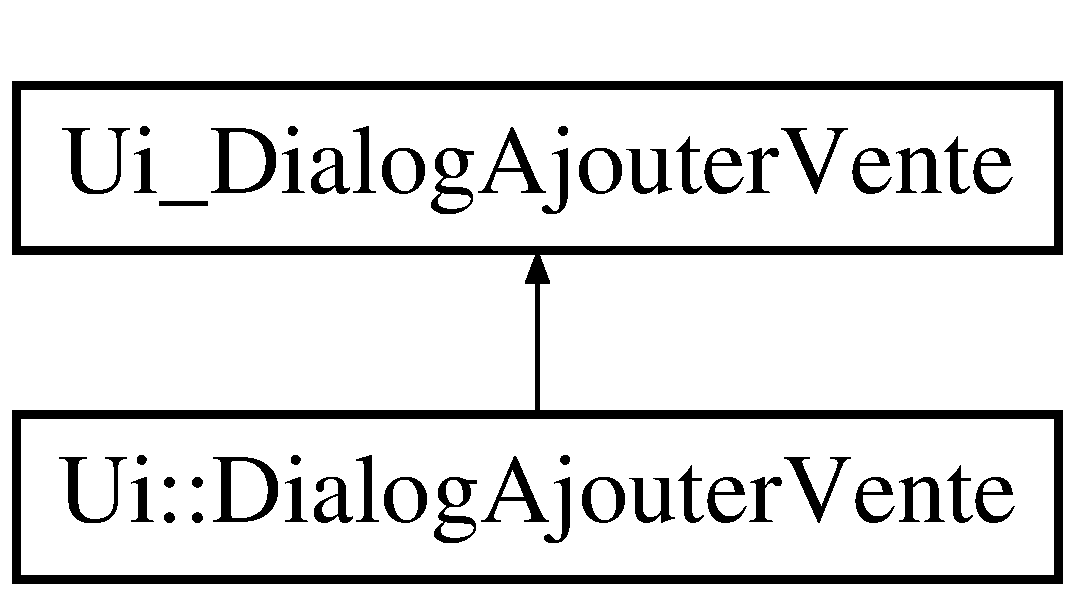
\includegraphics[height=2.000000cm]{class_ui___dialog_ajouter_vente}
\end{center}
\end{figure}
\subsection*{Fonctions membres publiques}
\begin{DoxyCompactItemize}
\item 
void \hyperlink{class_ui___dialog_ajouter_vente_ae883744c3e96eb7e48d7412542236d0b}{setup\-Ui} (Q\-Dialog $\ast$\hyperlink{class_dialog_ajouter_vente}{Dialog\-Ajouter\-Vente})
\item 
void \hyperlink{class_ui___dialog_ajouter_vente_ae2c336056d9da493f614411459dc933f}{retranslate\-Ui} (Q\-Dialog $\ast$\hyperlink{class_dialog_ajouter_vente}{Dialog\-Ajouter\-Vente})
\end{DoxyCompactItemize}
\subsection*{Attributs publics}
\begin{DoxyCompactItemize}
\item 
Q\-Label $\ast$ \hyperlink{class_ui___dialog_ajouter_vente_a0148c009801a386f05f72bb1eb85138a}{label}
\item 
Q\-Label $\ast$ \hyperlink{class_ui___dialog_ajouter_vente_a124aae2b361f68cd4e4999a4d5c81c36}{label\-Nom}
\item 
Q\-Line\-Edit $\ast$ \hyperlink{class_ui___dialog_ajouter_vente_a7f6dc97a576b62dc8412a347ec2acb25}{val\-Nom}
\item 
Q\-Label $\ast$ \hyperlink{class_ui___dialog_ajouter_vente_a1ad88f317080e18e9b9855589dc73ac1}{label\-Cat}
\item 
Q\-Line\-Edit $\ast$ \hyperlink{class_ui___dialog_ajouter_vente_a8fd18dbf5b8788ff61cad46e2bbf9cc0}{val\-Cat}
\item 
Q\-Label $\ast$ \hyperlink{class_ui___dialog_ajouter_vente_a2bc88408689024a4377bc0e2171c19d9}{label\-Prix}
\item 
Q\-Label $\ast$ \hyperlink{class_ui___dialog_ajouter_vente_a6c8d4acb3eea5f28abe8cee46319ff40}{label\-Qte}
\item 
Q\-Spin\-Box $\ast$ \hyperlink{class_ui___dialog_ajouter_vente_a763e8a0d9e253d6da640fbac8b02459c}{val\-Qte}
\item 
Q\-Label $\ast$ \hyperlink{class_ui___dialog_ajouter_vente_a3288030f764fff68a7e443c490fe969d}{label\-\_\-6}
\item 
Q\-Label $\ast$ \hyperlink{class_ui___dialog_ajouter_vente_adee51e354846fc85ed2a55004106373f}{label\-Date\-Limite}
\item 
Q\-Radio\-Button $\ast$ \hyperlink{class_ui___dialog_ajouter_vente_a6df6af19da8182b012f9ef7494eb8deb}{radio\-Enchere}
\item 
Q\-Date\-Edit $\ast$ \hyperlink{class_ui___dialog_ajouter_vente_a065ebc28106416bec403cecd4783c5c4}{val\-Date\-Limite}
\item 
Q\-Push\-Button $\ast$ \hyperlink{class_ui___dialog_ajouter_vente_a9b3dc0fa96393ccf69a41ae7776da8df}{bouton\-Ajouter\-Vente}
\item 
Q\-Radio\-Button $\ast$ \hyperlink{class_ui___dialog_ajouter_vente_a4ec0099d5d75035625d2f104a6882acc}{radio\-Normale}
\item 
Q\-Double\-Spin\-Box $\ast$ \hyperlink{class_ui___dialog_ajouter_vente_a125862f438ab182a8a49357a91bb37ef}{val\-Prix}
\item 
Q\-Button\-Group $\ast$ \hyperlink{class_ui___dialog_ajouter_vente_a7814de48092bce095428664bda3373d3}{button\-Group}
\end{DoxyCompactItemize}


\subsection{Documentation des fonctions membres}
\hypertarget{class_ui___dialog_ajouter_vente_ae2c336056d9da493f614411459dc933f}{\index{Ui\-\_\-\-Dialog\-Ajouter\-Vente@{Ui\-\_\-\-Dialog\-Ajouter\-Vente}!retranslate\-Ui@{retranslate\-Ui}}
\index{retranslate\-Ui@{retranslate\-Ui}!Ui_DialogAjouterVente@{Ui\-\_\-\-Dialog\-Ajouter\-Vente}}
\subsubsection[{retranslate\-Ui}]{\setlength{\rightskip}{0pt plus 5cm}void Ui\-\_\-\-Dialog\-Ajouter\-Vente\-::retranslate\-Ui (
\begin{DoxyParamCaption}
\item[{Q\-Dialog $\ast$}]{Dialog\-Ajouter\-Vente}
\end{DoxyParamCaption}
)\hspace{0.3cm}{\ttfamily [inline]}}}\label{class_ui___dialog_ajouter_vente_ae2c336056d9da493f614411459dc933f}
\hypertarget{class_ui___dialog_ajouter_vente_ae883744c3e96eb7e48d7412542236d0b}{\index{Ui\-\_\-\-Dialog\-Ajouter\-Vente@{Ui\-\_\-\-Dialog\-Ajouter\-Vente}!setup\-Ui@{setup\-Ui}}
\index{setup\-Ui@{setup\-Ui}!Ui_DialogAjouterVente@{Ui\-\_\-\-Dialog\-Ajouter\-Vente}}
\subsubsection[{setup\-Ui}]{\setlength{\rightskip}{0pt plus 5cm}void Ui\-\_\-\-Dialog\-Ajouter\-Vente\-::setup\-Ui (
\begin{DoxyParamCaption}
\item[{Q\-Dialog $\ast$}]{Dialog\-Ajouter\-Vente}
\end{DoxyParamCaption}
)\hspace{0.3cm}{\ttfamily [inline]}}}\label{class_ui___dialog_ajouter_vente_ae883744c3e96eb7e48d7412542236d0b}


\subsection{Documentation des données membres}
\hypertarget{class_ui___dialog_ajouter_vente_a9b3dc0fa96393ccf69a41ae7776da8df}{\index{Ui\-\_\-\-Dialog\-Ajouter\-Vente@{Ui\-\_\-\-Dialog\-Ajouter\-Vente}!bouton\-Ajouter\-Vente@{bouton\-Ajouter\-Vente}}
\index{bouton\-Ajouter\-Vente@{bouton\-Ajouter\-Vente}!Ui_DialogAjouterVente@{Ui\-\_\-\-Dialog\-Ajouter\-Vente}}
\subsubsection[{bouton\-Ajouter\-Vente}]{\setlength{\rightskip}{0pt plus 5cm}Q\-Push\-Button$\ast$ Ui\-\_\-\-Dialog\-Ajouter\-Vente\-::bouton\-Ajouter\-Vente}}\label{class_ui___dialog_ajouter_vente_a9b3dc0fa96393ccf69a41ae7776da8df}
\hypertarget{class_ui___dialog_ajouter_vente_a7814de48092bce095428664bda3373d3}{\index{Ui\-\_\-\-Dialog\-Ajouter\-Vente@{Ui\-\_\-\-Dialog\-Ajouter\-Vente}!button\-Group@{button\-Group}}
\index{button\-Group@{button\-Group}!Ui_DialogAjouterVente@{Ui\-\_\-\-Dialog\-Ajouter\-Vente}}
\subsubsection[{button\-Group}]{\setlength{\rightskip}{0pt plus 5cm}Q\-Button\-Group$\ast$ Ui\-\_\-\-Dialog\-Ajouter\-Vente\-::button\-Group}}\label{class_ui___dialog_ajouter_vente_a7814de48092bce095428664bda3373d3}
\hypertarget{class_ui___dialog_ajouter_vente_a0148c009801a386f05f72bb1eb85138a}{\index{Ui\-\_\-\-Dialog\-Ajouter\-Vente@{Ui\-\_\-\-Dialog\-Ajouter\-Vente}!label@{label}}
\index{label@{label}!Ui_DialogAjouterVente@{Ui\-\_\-\-Dialog\-Ajouter\-Vente}}
\subsubsection[{label}]{\setlength{\rightskip}{0pt plus 5cm}Q\-Label$\ast$ Ui\-\_\-\-Dialog\-Ajouter\-Vente\-::label}}\label{class_ui___dialog_ajouter_vente_a0148c009801a386f05f72bb1eb85138a}
\hypertarget{class_ui___dialog_ajouter_vente_a3288030f764fff68a7e443c490fe969d}{\index{Ui\-\_\-\-Dialog\-Ajouter\-Vente@{Ui\-\_\-\-Dialog\-Ajouter\-Vente}!label\-\_\-6@{label\-\_\-6}}
\index{label\-\_\-6@{label\-\_\-6}!Ui_DialogAjouterVente@{Ui\-\_\-\-Dialog\-Ajouter\-Vente}}
\subsubsection[{label\-\_\-6}]{\setlength{\rightskip}{0pt plus 5cm}Q\-Label$\ast$ Ui\-\_\-\-Dialog\-Ajouter\-Vente\-::label\-\_\-6}}\label{class_ui___dialog_ajouter_vente_a3288030f764fff68a7e443c490fe969d}
\hypertarget{class_ui___dialog_ajouter_vente_a1ad88f317080e18e9b9855589dc73ac1}{\index{Ui\-\_\-\-Dialog\-Ajouter\-Vente@{Ui\-\_\-\-Dialog\-Ajouter\-Vente}!label\-Cat@{label\-Cat}}
\index{label\-Cat@{label\-Cat}!Ui_DialogAjouterVente@{Ui\-\_\-\-Dialog\-Ajouter\-Vente}}
\subsubsection[{label\-Cat}]{\setlength{\rightskip}{0pt plus 5cm}Q\-Label$\ast$ Ui\-\_\-\-Dialog\-Ajouter\-Vente\-::label\-Cat}}\label{class_ui___dialog_ajouter_vente_a1ad88f317080e18e9b9855589dc73ac1}
\hypertarget{class_ui___dialog_ajouter_vente_adee51e354846fc85ed2a55004106373f}{\index{Ui\-\_\-\-Dialog\-Ajouter\-Vente@{Ui\-\_\-\-Dialog\-Ajouter\-Vente}!label\-Date\-Limite@{label\-Date\-Limite}}
\index{label\-Date\-Limite@{label\-Date\-Limite}!Ui_DialogAjouterVente@{Ui\-\_\-\-Dialog\-Ajouter\-Vente}}
\subsubsection[{label\-Date\-Limite}]{\setlength{\rightskip}{0pt plus 5cm}Q\-Label$\ast$ Ui\-\_\-\-Dialog\-Ajouter\-Vente\-::label\-Date\-Limite}}\label{class_ui___dialog_ajouter_vente_adee51e354846fc85ed2a55004106373f}
\hypertarget{class_ui___dialog_ajouter_vente_a124aae2b361f68cd4e4999a4d5c81c36}{\index{Ui\-\_\-\-Dialog\-Ajouter\-Vente@{Ui\-\_\-\-Dialog\-Ajouter\-Vente}!label\-Nom@{label\-Nom}}
\index{label\-Nom@{label\-Nom}!Ui_DialogAjouterVente@{Ui\-\_\-\-Dialog\-Ajouter\-Vente}}
\subsubsection[{label\-Nom}]{\setlength{\rightskip}{0pt plus 5cm}Q\-Label$\ast$ Ui\-\_\-\-Dialog\-Ajouter\-Vente\-::label\-Nom}}\label{class_ui___dialog_ajouter_vente_a124aae2b361f68cd4e4999a4d5c81c36}
\hypertarget{class_ui___dialog_ajouter_vente_a2bc88408689024a4377bc0e2171c19d9}{\index{Ui\-\_\-\-Dialog\-Ajouter\-Vente@{Ui\-\_\-\-Dialog\-Ajouter\-Vente}!label\-Prix@{label\-Prix}}
\index{label\-Prix@{label\-Prix}!Ui_DialogAjouterVente@{Ui\-\_\-\-Dialog\-Ajouter\-Vente}}
\subsubsection[{label\-Prix}]{\setlength{\rightskip}{0pt plus 5cm}Q\-Label$\ast$ Ui\-\_\-\-Dialog\-Ajouter\-Vente\-::label\-Prix}}\label{class_ui___dialog_ajouter_vente_a2bc88408689024a4377bc0e2171c19d9}
\hypertarget{class_ui___dialog_ajouter_vente_a6c8d4acb3eea5f28abe8cee46319ff40}{\index{Ui\-\_\-\-Dialog\-Ajouter\-Vente@{Ui\-\_\-\-Dialog\-Ajouter\-Vente}!label\-Qte@{label\-Qte}}
\index{label\-Qte@{label\-Qte}!Ui_DialogAjouterVente@{Ui\-\_\-\-Dialog\-Ajouter\-Vente}}
\subsubsection[{label\-Qte}]{\setlength{\rightskip}{0pt plus 5cm}Q\-Label$\ast$ Ui\-\_\-\-Dialog\-Ajouter\-Vente\-::label\-Qte}}\label{class_ui___dialog_ajouter_vente_a6c8d4acb3eea5f28abe8cee46319ff40}
\hypertarget{class_ui___dialog_ajouter_vente_a6df6af19da8182b012f9ef7494eb8deb}{\index{Ui\-\_\-\-Dialog\-Ajouter\-Vente@{Ui\-\_\-\-Dialog\-Ajouter\-Vente}!radio\-Enchere@{radio\-Enchere}}
\index{radio\-Enchere@{radio\-Enchere}!Ui_DialogAjouterVente@{Ui\-\_\-\-Dialog\-Ajouter\-Vente}}
\subsubsection[{radio\-Enchere}]{\setlength{\rightskip}{0pt plus 5cm}Q\-Radio\-Button$\ast$ Ui\-\_\-\-Dialog\-Ajouter\-Vente\-::radio\-Enchere}}\label{class_ui___dialog_ajouter_vente_a6df6af19da8182b012f9ef7494eb8deb}
\hypertarget{class_ui___dialog_ajouter_vente_a4ec0099d5d75035625d2f104a6882acc}{\index{Ui\-\_\-\-Dialog\-Ajouter\-Vente@{Ui\-\_\-\-Dialog\-Ajouter\-Vente}!radio\-Normale@{radio\-Normale}}
\index{radio\-Normale@{radio\-Normale}!Ui_DialogAjouterVente@{Ui\-\_\-\-Dialog\-Ajouter\-Vente}}
\subsubsection[{radio\-Normale}]{\setlength{\rightskip}{0pt plus 5cm}Q\-Radio\-Button$\ast$ Ui\-\_\-\-Dialog\-Ajouter\-Vente\-::radio\-Normale}}\label{class_ui___dialog_ajouter_vente_a4ec0099d5d75035625d2f104a6882acc}
\hypertarget{class_ui___dialog_ajouter_vente_a8fd18dbf5b8788ff61cad46e2bbf9cc0}{\index{Ui\-\_\-\-Dialog\-Ajouter\-Vente@{Ui\-\_\-\-Dialog\-Ajouter\-Vente}!val\-Cat@{val\-Cat}}
\index{val\-Cat@{val\-Cat}!Ui_DialogAjouterVente@{Ui\-\_\-\-Dialog\-Ajouter\-Vente}}
\subsubsection[{val\-Cat}]{\setlength{\rightskip}{0pt plus 5cm}Q\-Line\-Edit$\ast$ Ui\-\_\-\-Dialog\-Ajouter\-Vente\-::val\-Cat}}\label{class_ui___dialog_ajouter_vente_a8fd18dbf5b8788ff61cad46e2bbf9cc0}
\hypertarget{class_ui___dialog_ajouter_vente_a065ebc28106416bec403cecd4783c5c4}{\index{Ui\-\_\-\-Dialog\-Ajouter\-Vente@{Ui\-\_\-\-Dialog\-Ajouter\-Vente}!val\-Date\-Limite@{val\-Date\-Limite}}
\index{val\-Date\-Limite@{val\-Date\-Limite}!Ui_DialogAjouterVente@{Ui\-\_\-\-Dialog\-Ajouter\-Vente}}
\subsubsection[{val\-Date\-Limite}]{\setlength{\rightskip}{0pt plus 5cm}Q\-Date\-Edit$\ast$ Ui\-\_\-\-Dialog\-Ajouter\-Vente\-::val\-Date\-Limite}}\label{class_ui___dialog_ajouter_vente_a065ebc28106416bec403cecd4783c5c4}
\hypertarget{class_ui___dialog_ajouter_vente_a7f6dc97a576b62dc8412a347ec2acb25}{\index{Ui\-\_\-\-Dialog\-Ajouter\-Vente@{Ui\-\_\-\-Dialog\-Ajouter\-Vente}!val\-Nom@{val\-Nom}}
\index{val\-Nom@{val\-Nom}!Ui_DialogAjouterVente@{Ui\-\_\-\-Dialog\-Ajouter\-Vente}}
\subsubsection[{val\-Nom}]{\setlength{\rightskip}{0pt plus 5cm}Q\-Line\-Edit$\ast$ Ui\-\_\-\-Dialog\-Ajouter\-Vente\-::val\-Nom}}\label{class_ui___dialog_ajouter_vente_a7f6dc97a576b62dc8412a347ec2acb25}
\hypertarget{class_ui___dialog_ajouter_vente_a125862f438ab182a8a49357a91bb37ef}{\index{Ui\-\_\-\-Dialog\-Ajouter\-Vente@{Ui\-\_\-\-Dialog\-Ajouter\-Vente}!val\-Prix@{val\-Prix}}
\index{val\-Prix@{val\-Prix}!Ui_DialogAjouterVente@{Ui\-\_\-\-Dialog\-Ajouter\-Vente}}
\subsubsection[{val\-Prix}]{\setlength{\rightskip}{0pt plus 5cm}Q\-Double\-Spin\-Box$\ast$ Ui\-\_\-\-Dialog\-Ajouter\-Vente\-::val\-Prix}}\label{class_ui___dialog_ajouter_vente_a125862f438ab182a8a49357a91bb37ef}
\hypertarget{class_ui___dialog_ajouter_vente_a763e8a0d9e253d6da640fbac8b02459c}{\index{Ui\-\_\-\-Dialog\-Ajouter\-Vente@{Ui\-\_\-\-Dialog\-Ajouter\-Vente}!val\-Qte@{val\-Qte}}
\index{val\-Qte@{val\-Qte}!Ui_DialogAjouterVente@{Ui\-\_\-\-Dialog\-Ajouter\-Vente}}
\subsubsection[{val\-Qte}]{\setlength{\rightskip}{0pt plus 5cm}Q\-Spin\-Box$\ast$ Ui\-\_\-\-Dialog\-Ajouter\-Vente\-::val\-Qte}}\label{class_ui___dialog_ajouter_vente_a763e8a0d9e253d6da640fbac8b02459c}


La documentation de cette classe a été générée à partir du fichier suivant \-:\begin{DoxyCompactItemize}
\item 
/home/magalie/\-Bureau/\-S5/\-C\-P\-O\-O\-A/\-Projet/\-E-\/\-Marche-\//iterations/iteration4/\-E\-Marche/\hyperlink{ui___dialog_ajouter_vente_8h}{ui\-\_\-\-Dialog\-Ajouter\-Vente.\-h}\end{DoxyCompactItemize}

\hypertarget{class_ui___dialog_connexion}{\section{Référence de la classe Ui\-\_\-\-Dialog\-Connexion}
\label{class_ui___dialog_connexion}\index{Ui\-\_\-\-Dialog\-Connexion@{Ui\-\_\-\-Dialog\-Connexion}}
}


{\ttfamily \#include $<$ui\-\_\-\-Dialog\-Connexion.\-h$>$}

Graphe d'héritage de Ui\-\_\-\-Dialog\-Connexion\-:\begin{figure}[H]
\begin{center}
\leavevmode
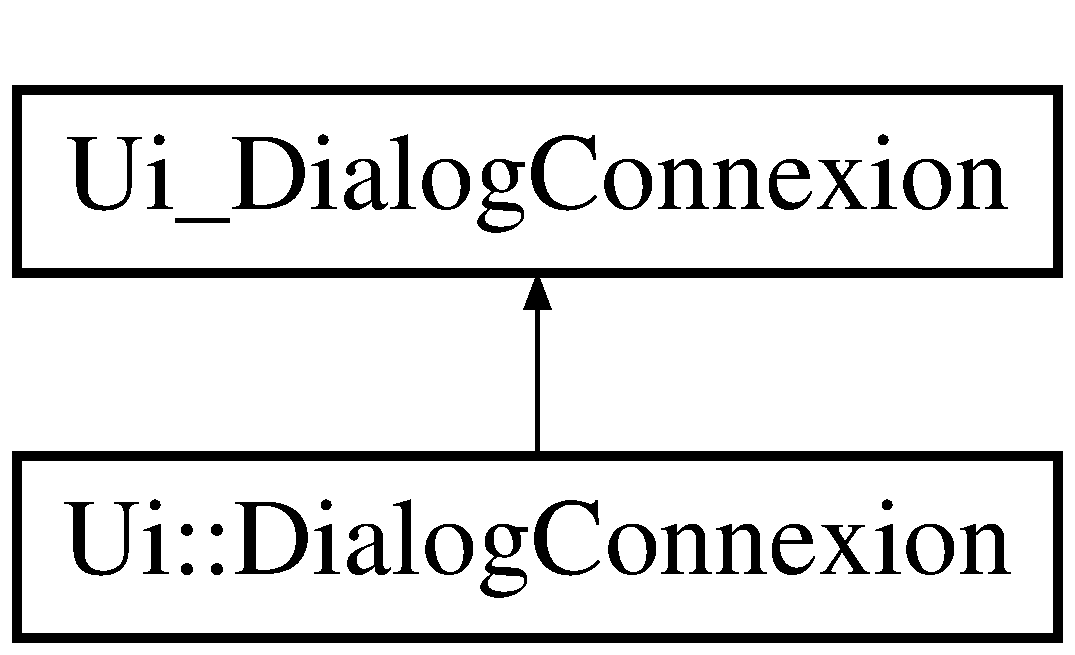
\includegraphics[height=2.000000cm]{class_ui___dialog_connexion}
\end{center}
\end{figure}
\subsection*{Fonctions membres publiques}
\begin{DoxyCompactItemize}
\item 
void \hyperlink{class_ui___dialog_connexion_a6291dbf1c6dca03c2a9e70d87007b113}{setup\-Ui} (Q\-Dialog $\ast$\hyperlink{class_dialog_connexion}{Dialog\-Connexion})
\item 
void \hyperlink{class_ui___dialog_connexion_a3c9e6d3213c98a4c3d21bb365e87f79c}{retranslate\-Ui} (Q\-Dialog $\ast$\hyperlink{class_dialog_connexion}{Dialog\-Connexion})
\end{DoxyCompactItemize}
\subsection*{Attributs publics}
\begin{DoxyCompactItemize}
\item 
Q\-Label $\ast$ \hyperlink{class_ui___dialog_connexion_ad90d75071d6c9d6e5539a7115156f5eb}{label\-Connexion}
\item 
Q\-Push\-Button $\ast$ \hyperlink{class_ui___dialog_connexion_a5c7679d0477929e0d177aa38f9277f62}{bouton\-Se\-Connecter}
\item 
Q\-Push\-Button $\ast$ \hyperlink{class_ui___dialog_connexion_a11208b09a06acbe25a6c352bdd4c0b3b}{bouton\-S\-Inscrire}
\item 
Q\-Widget $\ast$ \hyperlink{class_ui___dialog_connexion_afeb60fc13dde76b19301251dddc60e21}{layout\-Widget}
\item 
Q\-Form\-Layout $\ast$ \hyperlink{class_ui___dialog_connexion_aeddc51c77c362a789e75246e03e62713}{form\-Layout}
\item 
Q\-Label $\ast$ \hyperlink{class_ui___dialog_connexion_a10c9345fc39e8cc6c73531d688ff13ae}{label\-Pseudo}
\item 
Q\-Line\-Edit $\ast$ \hyperlink{class_ui___dialog_connexion_a4560ad500c66e02c38d52f01b71c5c8b}{val\-Pseudo}
\item 
Q\-Widget $\ast$ \hyperlink{class_ui___dialog_connexion_a89b895d2240121522d39f47995075b71}{layout\-Widget1}
\item 
Q\-Form\-Layout $\ast$ \hyperlink{class_ui___dialog_connexion_ad824817e926068b482b4bf73f9632086}{form\-Layout\-\_\-2}
\item 
Q\-Label $\ast$ \hyperlink{class_ui___dialog_connexion_aa6e5c9b46e3423bd6427192e6fd499a1}{label\-Mdp}
\item 
Q\-Line\-Edit $\ast$ \hyperlink{class_ui___dialog_connexion_ae59151879eebdd101eaae39a532cdff8}{val\-Mdp}
\end{DoxyCompactItemize}


\subsection{Documentation des fonctions membres}
\hypertarget{class_ui___dialog_connexion_a3c9e6d3213c98a4c3d21bb365e87f79c}{\index{Ui\-\_\-\-Dialog\-Connexion@{Ui\-\_\-\-Dialog\-Connexion}!retranslate\-Ui@{retranslate\-Ui}}
\index{retranslate\-Ui@{retranslate\-Ui}!Ui_DialogConnexion@{Ui\-\_\-\-Dialog\-Connexion}}
\subsubsection[{retranslate\-Ui}]{\setlength{\rightskip}{0pt plus 5cm}void Ui\-\_\-\-Dialog\-Connexion\-::retranslate\-Ui (
\begin{DoxyParamCaption}
\item[{Q\-Dialog $\ast$}]{Dialog\-Connexion}
\end{DoxyParamCaption}
)\hspace{0.3cm}{\ttfamily [inline]}}}\label{class_ui___dialog_connexion_a3c9e6d3213c98a4c3d21bb365e87f79c}
\hypertarget{class_ui___dialog_connexion_a6291dbf1c6dca03c2a9e70d87007b113}{\index{Ui\-\_\-\-Dialog\-Connexion@{Ui\-\_\-\-Dialog\-Connexion}!setup\-Ui@{setup\-Ui}}
\index{setup\-Ui@{setup\-Ui}!Ui_DialogConnexion@{Ui\-\_\-\-Dialog\-Connexion}}
\subsubsection[{setup\-Ui}]{\setlength{\rightskip}{0pt plus 5cm}void Ui\-\_\-\-Dialog\-Connexion\-::setup\-Ui (
\begin{DoxyParamCaption}
\item[{Q\-Dialog $\ast$}]{Dialog\-Connexion}
\end{DoxyParamCaption}
)\hspace{0.3cm}{\ttfamily [inline]}}}\label{class_ui___dialog_connexion_a6291dbf1c6dca03c2a9e70d87007b113}


\subsection{Documentation des données membres}
\hypertarget{class_ui___dialog_connexion_a5c7679d0477929e0d177aa38f9277f62}{\index{Ui\-\_\-\-Dialog\-Connexion@{Ui\-\_\-\-Dialog\-Connexion}!bouton\-Se\-Connecter@{bouton\-Se\-Connecter}}
\index{bouton\-Se\-Connecter@{bouton\-Se\-Connecter}!Ui_DialogConnexion@{Ui\-\_\-\-Dialog\-Connexion}}
\subsubsection[{bouton\-Se\-Connecter}]{\setlength{\rightskip}{0pt plus 5cm}Q\-Push\-Button$\ast$ Ui\-\_\-\-Dialog\-Connexion\-::bouton\-Se\-Connecter}}\label{class_ui___dialog_connexion_a5c7679d0477929e0d177aa38f9277f62}
\hypertarget{class_ui___dialog_connexion_a11208b09a06acbe25a6c352bdd4c0b3b}{\index{Ui\-\_\-\-Dialog\-Connexion@{Ui\-\_\-\-Dialog\-Connexion}!bouton\-S\-Inscrire@{bouton\-S\-Inscrire}}
\index{bouton\-S\-Inscrire@{bouton\-S\-Inscrire}!Ui_DialogConnexion@{Ui\-\_\-\-Dialog\-Connexion}}
\subsubsection[{bouton\-S\-Inscrire}]{\setlength{\rightskip}{0pt plus 5cm}Q\-Push\-Button$\ast$ Ui\-\_\-\-Dialog\-Connexion\-::bouton\-S\-Inscrire}}\label{class_ui___dialog_connexion_a11208b09a06acbe25a6c352bdd4c0b3b}
\hypertarget{class_ui___dialog_connexion_aeddc51c77c362a789e75246e03e62713}{\index{Ui\-\_\-\-Dialog\-Connexion@{Ui\-\_\-\-Dialog\-Connexion}!form\-Layout@{form\-Layout}}
\index{form\-Layout@{form\-Layout}!Ui_DialogConnexion@{Ui\-\_\-\-Dialog\-Connexion}}
\subsubsection[{form\-Layout}]{\setlength{\rightskip}{0pt plus 5cm}Q\-Form\-Layout$\ast$ Ui\-\_\-\-Dialog\-Connexion\-::form\-Layout}}\label{class_ui___dialog_connexion_aeddc51c77c362a789e75246e03e62713}
\hypertarget{class_ui___dialog_connexion_ad824817e926068b482b4bf73f9632086}{\index{Ui\-\_\-\-Dialog\-Connexion@{Ui\-\_\-\-Dialog\-Connexion}!form\-Layout\-\_\-2@{form\-Layout\-\_\-2}}
\index{form\-Layout\-\_\-2@{form\-Layout\-\_\-2}!Ui_DialogConnexion@{Ui\-\_\-\-Dialog\-Connexion}}
\subsubsection[{form\-Layout\-\_\-2}]{\setlength{\rightskip}{0pt plus 5cm}Q\-Form\-Layout$\ast$ Ui\-\_\-\-Dialog\-Connexion\-::form\-Layout\-\_\-2}}\label{class_ui___dialog_connexion_ad824817e926068b482b4bf73f9632086}
\hypertarget{class_ui___dialog_connexion_ad90d75071d6c9d6e5539a7115156f5eb}{\index{Ui\-\_\-\-Dialog\-Connexion@{Ui\-\_\-\-Dialog\-Connexion}!label\-Connexion@{label\-Connexion}}
\index{label\-Connexion@{label\-Connexion}!Ui_DialogConnexion@{Ui\-\_\-\-Dialog\-Connexion}}
\subsubsection[{label\-Connexion}]{\setlength{\rightskip}{0pt plus 5cm}Q\-Label$\ast$ Ui\-\_\-\-Dialog\-Connexion\-::label\-Connexion}}\label{class_ui___dialog_connexion_ad90d75071d6c9d6e5539a7115156f5eb}
\hypertarget{class_ui___dialog_connexion_aa6e5c9b46e3423bd6427192e6fd499a1}{\index{Ui\-\_\-\-Dialog\-Connexion@{Ui\-\_\-\-Dialog\-Connexion}!label\-Mdp@{label\-Mdp}}
\index{label\-Mdp@{label\-Mdp}!Ui_DialogConnexion@{Ui\-\_\-\-Dialog\-Connexion}}
\subsubsection[{label\-Mdp}]{\setlength{\rightskip}{0pt plus 5cm}Q\-Label$\ast$ Ui\-\_\-\-Dialog\-Connexion\-::label\-Mdp}}\label{class_ui___dialog_connexion_aa6e5c9b46e3423bd6427192e6fd499a1}
\hypertarget{class_ui___dialog_connexion_a10c9345fc39e8cc6c73531d688ff13ae}{\index{Ui\-\_\-\-Dialog\-Connexion@{Ui\-\_\-\-Dialog\-Connexion}!label\-Pseudo@{label\-Pseudo}}
\index{label\-Pseudo@{label\-Pseudo}!Ui_DialogConnexion@{Ui\-\_\-\-Dialog\-Connexion}}
\subsubsection[{label\-Pseudo}]{\setlength{\rightskip}{0pt plus 5cm}Q\-Label$\ast$ Ui\-\_\-\-Dialog\-Connexion\-::label\-Pseudo}}\label{class_ui___dialog_connexion_a10c9345fc39e8cc6c73531d688ff13ae}
\hypertarget{class_ui___dialog_connexion_afeb60fc13dde76b19301251dddc60e21}{\index{Ui\-\_\-\-Dialog\-Connexion@{Ui\-\_\-\-Dialog\-Connexion}!layout\-Widget@{layout\-Widget}}
\index{layout\-Widget@{layout\-Widget}!Ui_DialogConnexion@{Ui\-\_\-\-Dialog\-Connexion}}
\subsubsection[{layout\-Widget}]{\setlength{\rightskip}{0pt plus 5cm}Q\-Widget$\ast$ Ui\-\_\-\-Dialog\-Connexion\-::layout\-Widget}}\label{class_ui___dialog_connexion_afeb60fc13dde76b19301251dddc60e21}
\hypertarget{class_ui___dialog_connexion_a89b895d2240121522d39f47995075b71}{\index{Ui\-\_\-\-Dialog\-Connexion@{Ui\-\_\-\-Dialog\-Connexion}!layout\-Widget1@{layout\-Widget1}}
\index{layout\-Widget1@{layout\-Widget1}!Ui_DialogConnexion@{Ui\-\_\-\-Dialog\-Connexion}}
\subsubsection[{layout\-Widget1}]{\setlength{\rightskip}{0pt plus 5cm}Q\-Widget$\ast$ Ui\-\_\-\-Dialog\-Connexion\-::layout\-Widget1}}\label{class_ui___dialog_connexion_a89b895d2240121522d39f47995075b71}
\hypertarget{class_ui___dialog_connexion_ae59151879eebdd101eaae39a532cdff8}{\index{Ui\-\_\-\-Dialog\-Connexion@{Ui\-\_\-\-Dialog\-Connexion}!val\-Mdp@{val\-Mdp}}
\index{val\-Mdp@{val\-Mdp}!Ui_DialogConnexion@{Ui\-\_\-\-Dialog\-Connexion}}
\subsubsection[{val\-Mdp}]{\setlength{\rightskip}{0pt plus 5cm}Q\-Line\-Edit$\ast$ Ui\-\_\-\-Dialog\-Connexion\-::val\-Mdp}}\label{class_ui___dialog_connexion_ae59151879eebdd101eaae39a532cdff8}
\hypertarget{class_ui___dialog_connexion_a4560ad500c66e02c38d52f01b71c5c8b}{\index{Ui\-\_\-\-Dialog\-Connexion@{Ui\-\_\-\-Dialog\-Connexion}!val\-Pseudo@{val\-Pseudo}}
\index{val\-Pseudo@{val\-Pseudo}!Ui_DialogConnexion@{Ui\-\_\-\-Dialog\-Connexion}}
\subsubsection[{val\-Pseudo}]{\setlength{\rightskip}{0pt plus 5cm}Q\-Line\-Edit$\ast$ Ui\-\_\-\-Dialog\-Connexion\-::val\-Pseudo}}\label{class_ui___dialog_connexion_a4560ad500c66e02c38d52f01b71c5c8b}


La documentation de cette classe a été générée à partir du fichier suivant \-:\begin{DoxyCompactItemize}
\item 
/home/magalie/\-Bureau/\-S5/\-C\-P\-O\-O\-A/\-Projet/\-E-\/\-Marche-\//iterations/iteration2/\-E\-Marche/\hyperlink{ui___dialog_connexion_8h}{ui\-\_\-\-Dialog\-Connexion.\-h}\end{DoxyCompactItemize}

\hypertarget{class_ui___dialog_inscription}{\section{Référence de la classe Ui\-\_\-\-Dialog\-Inscription}
\label{class_ui___dialog_inscription}\index{Ui\-\_\-\-Dialog\-Inscription@{Ui\-\_\-\-Dialog\-Inscription}}
}


{\ttfamily \#include $<$ui\-\_\-\-Dialog\-Inscription.\-h$>$}

Graphe d'héritage de Ui\-\_\-\-Dialog\-Inscription\-:\begin{figure}[H]
\begin{center}
\leavevmode
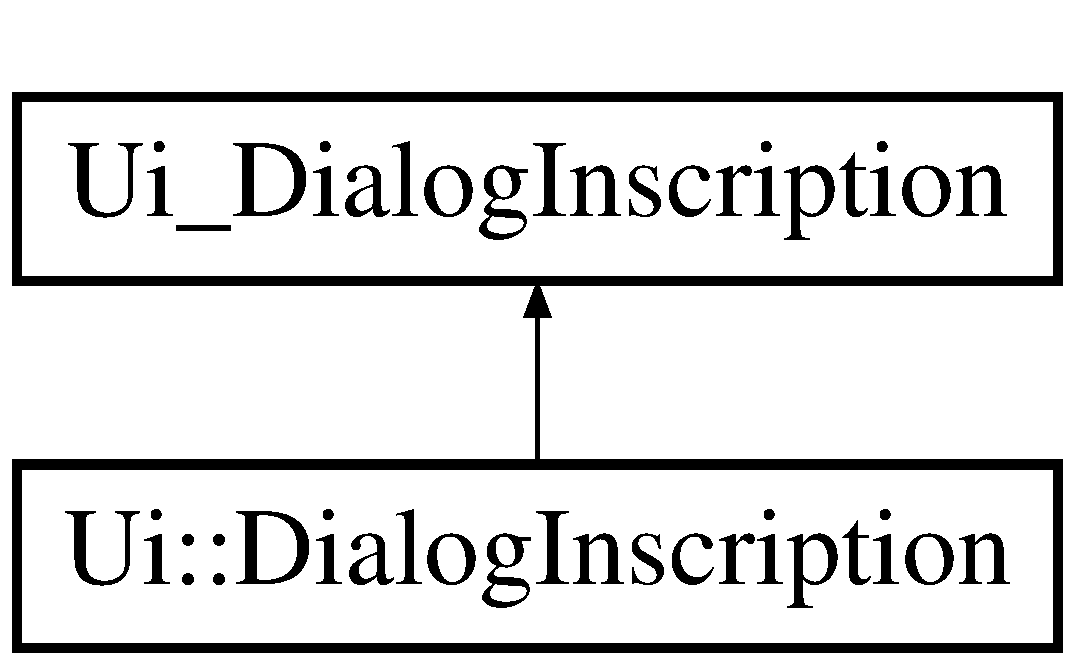
\includegraphics[height=2.000000cm]{class_ui___dialog_inscription}
\end{center}
\end{figure}
\subsection*{Fonctions membres publiques}
\begin{DoxyCompactItemize}
\item 
void \hyperlink{class_ui___dialog_inscription_aac8f38192f3e2691f410ae201df0d742}{setup\-Ui} (Q\-Dialog $\ast$Dialog\-Inscription)
\item 
void \hyperlink{class_ui___dialog_inscription_ae1af8d7775047088b4a14746e457b66e}{retranslate\-Ui} (Q\-Dialog $\ast$Dialog\-Inscription)
\end{DoxyCompactItemize}
\subsection*{Attributs publics}
\begin{DoxyCompactItemize}
\item 
Q\-Label $\ast$ \hyperlink{class_ui___dialog_inscription_ad6cbb361ce390cc8ebf99e4774d5b21d}{label\-Pseudo}
\item 
Q\-Line\-Edit $\ast$ \hyperlink{class_ui___dialog_inscription_a5893587115e987676400b0a5912ef6a8}{val\-Pseudo}
\item 
Q\-Label $\ast$ \hyperlink{class_ui___dialog_inscription_a3a3bb8c1384c3ddc6e30cce2d5f006be}{label\-Mdp}
\item 
Q\-Line\-Edit $\ast$ \hyperlink{class_ui___dialog_inscription_aecfee6e95908c76088f926cc4273c661}{val\-Mdp}
\item 
Q\-Label $\ast$ \hyperlink{class_ui___dialog_inscription_a40577873306a0cff844f092596900be6}{label\-Mdp2}
\item 
Q\-Line\-Edit $\ast$ \hyperlink{class_ui___dialog_inscription_aeaf99f06b2313bebaa084ff3b962b377}{val\-Mdp2}
\item 
Q\-Label $\ast$ \hyperlink{class_ui___dialog_inscription_a37335311fc697d84e29041a28c0b3a16}{label\-Nom}
\item 
Q\-Line\-Edit $\ast$ \hyperlink{class_ui___dialog_inscription_a5f1ec1d09785e1f5da1d3d436a9a4e00}{val\-Nom}
\item 
Q\-Label $\ast$ \hyperlink{class_ui___dialog_inscription_a90652e248fbff5e80d7ae7f465f3c67a}{label\-Prenom}
\item 
Q\-Line\-Edit $\ast$ \hyperlink{class_ui___dialog_inscription_a9fcf8c25b58d8d186801291b351f71a6}{val\-Prenom}
\item 
Q\-Label $\ast$ \hyperlink{class_ui___dialog_inscription_aa8405fd8a2dba259c85174fbd1815025}{label\-Mail}
\item 
Q\-Line\-Edit $\ast$ \hyperlink{class_ui___dialog_inscription_a620d0c3971f7a8134de43c5cb4141d0b}{val\-Mail}
\item 
Q\-Label $\ast$ \hyperlink{class_ui___dialog_inscription_a83b16295a5660be94337009689309625}{label\-Mail2}
\item 
Q\-Line\-Edit $\ast$ \hyperlink{class_ui___dialog_inscription_a2117b03c051572a35de79494744e2161}{val\-Mail2}
\item 
Q\-Label $\ast$ \hyperlink{class_ui___dialog_inscription_a41ff3fa5247196c1a310781633672ea7}{label\-Date\-Naissance}
\item 
Q\-Label $\ast$ \hyperlink{class_ui___dialog_inscription_ad5bb5ca7f98ec799abd4a83c56fff220}{label\-Adresse}
\item 
Q\-Line\-Edit $\ast$ \hyperlink{class_ui___dialog_inscription_ac5ffebadc65a04992a0c00ffcdd8378c}{val\-Adresse}
\item 
Q\-Label $\ast$ \hyperlink{class_ui___dialog_inscription_a8f0a88b8bbc71f40331af3dc6672b605}{label\-Code\-Postal}
\item 
Q\-Line\-Edit $\ast$ \hyperlink{class_ui___dialog_inscription_a3f257084e12a690ae6424651f2ca0906}{val\-Code\-Postal}
\item 
Q\-Label $\ast$ \hyperlink{class_ui___dialog_inscription_a21cf68832bf725cc2cb702a5d4338173}{label\-Ville}
\item 
Q\-Line\-Edit $\ast$ \hyperlink{class_ui___dialog_inscription_a97278f7c4479f5eebee4d44527362cd5}{val\-Ville}
\item 
Q\-Label $\ast$ \hyperlink{class_ui___dialog_inscription_a452e0b0adff0141927a345e5c92ca4b1}{label\-Inscription}
\item 
Q\-Push\-Button $\ast$ \hyperlink{class_ui___dialog_inscription_abcf7cc88e00f9004f42b1bea602d584a}{bouton\-Valider}
\item 
Q\-Date\-Edit $\ast$ \hyperlink{class_ui___dialog_inscription_a275d934e6e7ad6848d05f4f92fb28289}{val\-Date\-Naissance}
\end{DoxyCompactItemize}


\subsection{Documentation des fonctions membres}
\hypertarget{class_ui___dialog_inscription_ae1af8d7775047088b4a14746e457b66e}{\index{Ui\-\_\-\-Dialog\-Inscription@{Ui\-\_\-\-Dialog\-Inscription}!retranslate\-Ui@{retranslate\-Ui}}
\index{retranslate\-Ui@{retranslate\-Ui}!Ui_DialogInscription@{Ui\-\_\-\-Dialog\-Inscription}}
\subsubsection[{retranslate\-Ui}]{\setlength{\rightskip}{0pt plus 5cm}void Ui\-\_\-\-Dialog\-Inscription\-::retranslate\-Ui (
\begin{DoxyParamCaption}
\item[{Q\-Dialog $\ast$}]{Dialog\-Inscription}
\end{DoxyParamCaption}
)\hspace{0.3cm}{\ttfamily [inline]}}}\label{class_ui___dialog_inscription_ae1af8d7775047088b4a14746e457b66e}
\hypertarget{class_ui___dialog_inscription_aac8f38192f3e2691f410ae201df0d742}{\index{Ui\-\_\-\-Dialog\-Inscription@{Ui\-\_\-\-Dialog\-Inscription}!setup\-Ui@{setup\-Ui}}
\index{setup\-Ui@{setup\-Ui}!Ui_DialogInscription@{Ui\-\_\-\-Dialog\-Inscription}}
\subsubsection[{setup\-Ui}]{\setlength{\rightskip}{0pt plus 5cm}void Ui\-\_\-\-Dialog\-Inscription\-::setup\-Ui (
\begin{DoxyParamCaption}
\item[{Q\-Dialog $\ast$}]{Dialog\-Inscription}
\end{DoxyParamCaption}
)\hspace{0.3cm}{\ttfamily [inline]}}}\label{class_ui___dialog_inscription_aac8f38192f3e2691f410ae201df0d742}


\subsection{Documentation des données membres}
\hypertarget{class_ui___dialog_inscription_abcf7cc88e00f9004f42b1bea602d584a}{\index{Ui\-\_\-\-Dialog\-Inscription@{Ui\-\_\-\-Dialog\-Inscription}!bouton\-Valider@{bouton\-Valider}}
\index{bouton\-Valider@{bouton\-Valider}!Ui_DialogInscription@{Ui\-\_\-\-Dialog\-Inscription}}
\subsubsection[{bouton\-Valider}]{\setlength{\rightskip}{0pt plus 5cm}Q\-Push\-Button$\ast$ Ui\-\_\-\-Dialog\-Inscription\-::bouton\-Valider}}\label{class_ui___dialog_inscription_abcf7cc88e00f9004f42b1bea602d584a}
\hypertarget{class_ui___dialog_inscription_ad5bb5ca7f98ec799abd4a83c56fff220}{\index{Ui\-\_\-\-Dialog\-Inscription@{Ui\-\_\-\-Dialog\-Inscription}!label\-Adresse@{label\-Adresse}}
\index{label\-Adresse@{label\-Adresse}!Ui_DialogInscription@{Ui\-\_\-\-Dialog\-Inscription}}
\subsubsection[{label\-Adresse}]{\setlength{\rightskip}{0pt plus 5cm}Q\-Label$\ast$ Ui\-\_\-\-Dialog\-Inscription\-::label\-Adresse}}\label{class_ui___dialog_inscription_ad5bb5ca7f98ec799abd4a83c56fff220}
\hypertarget{class_ui___dialog_inscription_a8f0a88b8bbc71f40331af3dc6672b605}{\index{Ui\-\_\-\-Dialog\-Inscription@{Ui\-\_\-\-Dialog\-Inscription}!label\-Code\-Postal@{label\-Code\-Postal}}
\index{label\-Code\-Postal@{label\-Code\-Postal}!Ui_DialogInscription@{Ui\-\_\-\-Dialog\-Inscription}}
\subsubsection[{label\-Code\-Postal}]{\setlength{\rightskip}{0pt plus 5cm}Q\-Label$\ast$ Ui\-\_\-\-Dialog\-Inscription\-::label\-Code\-Postal}}\label{class_ui___dialog_inscription_a8f0a88b8bbc71f40331af3dc6672b605}
\hypertarget{class_ui___dialog_inscription_a41ff3fa5247196c1a310781633672ea7}{\index{Ui\-\_\-\-Dialog\-Inscription@{Ui\-\_\-\-Dialog\-Inscription}!label\-Date\-Naissance@{label\-Date\-Naissance}}
\index{label\-Date\-Naissance@{label\-Date\-Naissance}!Ui_DialogInscription@{Ui\-\_\-\-Dialog\-Inscription}}
\subsubsection[{label\-Date\-Naissance}]{\setlength{\rightskip}{0pt plus 5cm}Q\-Label$\ast$ Ui\-\_\-\-Dialog\-Inscription\-::label\-Date\-Naissance}}\label{class_ui___dialog_inscription_a41ff3fa5247196c1a310781633672ea7}
\hypertarget{class_ui___dialog_inscription_a452e0b0adff0141927a345e5c92ca4b1}{\index{Ui\-\_\-\-Dialog\-Inscription@{Ui\-\_\-\-Dialog\-Inscription}!label\-Inscription@{label\-Inscription}}
\index{label\-Inscription@{label\-Inscription}!Ui_DialogInscription@{Ui\-\_\-\-Dialog\-Inscription}}
\subsubsection[{label\-Inscription}]{\setlength{\rightskip}{0pt plus 5cm}Q\-Label$\ast$ Ui\-\_\-\-Dialog\-Inscription\-::label\-Inscription}}\label{class_ui___dialog_inscription_a452e0b0adff0141927a345e5c92ca4b1}
\hypertarget{class_ui___dialog_inscription_aa8405fd8a2dba259c85174fbd1815025}{\index{Ui\-\_\-\-Dialog\-Inscription@{Ui\-\_\-\-Dialog\-Inscription}!label\-Mail@{label\-Mail}}
\index{label\-Mail@{label\-Mail}!Ui_DialogInscription@{Ui\-\_\-\-Dialog\-Inscription}}
\subsubsection[{label\-Mail}]{\setlength{\rightskip}{0pt plus 5cm}Q\-Label$\ast$ Ui\-\_\-\-Dialog\-Inscription\-::label\-Mail}}\label{class_ui___dialog_inscription_aa8405fd8a2dba259c85174fbd1815025}
\hypertarget{class_ui___dialog_inscription_a83b16295a5660be94337009689309625}{\index{Ui\-\_\-\-Dialog\-Inscription@{Ui\-\_\-\-Dialog\-Inscription}!label\-Mail2@{label\-Mail2}}
\index{label\-Mail2@{label\-Mail2}!Ui_DialogInscription@{Ui\-\_\-\-Dialog\-Inscription}}
\subsubsection[{label\-Mail2}]{\setlength{\rightskip}{0pt plus 5cm}Q\-Label$\ast$ Ui\-\_\-\-Dialog\-Inscription\-::label\-Mail2}}\label{class_ui___dialog_inscription_a83b16295a5660be94337009689309625}
\hypertarget{class_ui___dialog_inscription_a3a3bb8c1384c3ddc6e30cce2d5f006be}{\index{Ui\-\_\-\-Dialog\-Inscription@{Ui\-\_\-\-Dialog\-Inscription}!label\-Mdp@{label\-Mdp}}
\index{label\-Mdp@{label\-Mdp}!Ui_DialogInscription@{Ui\-\_\-\-Dialog\-Inscription}}
\subsubsection[{label\-Mdp}]{\setlength{\rightskip}{0pt plus 5cm}Q\-Label$\ast$ Ui\-\_\-\-Dialog\-Inscription\-::label\-Mdp}}\label{class_ui___dialog_inscription_a3a3bb8c1384c3ddc6e30cce2d5f006be}
\hypertarget{class_ui___dialog_inscription_a40577873306a0cff844f092596900be6}{\index{Ui\-\_\-\-Dialog\-Inscription@{Ui\-\_\-\-Dialog\-Inscription}!label\-Mdp2@{label\-Mdp2}}
\index{label\-Mdp2@{label\-Mdp2}!Ui_DialogInscription@{Ui\-\_\-\-Dialog\-Inscription}}
\subsubsection[{label\-Mdp2}]{\setlength{\rightskip}{0pt plus 5cm}Q\-Label$\ast$ Ui\-\_\-\-Dialog\-Inscription\-::label\-Mdp2}}\label{class_ui___dialog_inscription_a40577873306a0cff844f092596900be6}
\hypertarget{class_ui___dialog_inscription_a37335311fc697d84e29041a28c0b3a16}{\index{Ui\-\_\-\-Dialog\-Inscription@{Ui\-\_\-\-Dialog\-Inscription}!label\-Nom@{label\-Nom}}
\index{label\-Nom@{label\-Nom}!Ui_DialogInscription@{Ui\-\_\-\-Dialog\-Inscription}}
\subsubsection[{label\-Nom}]{\setlength{\rightskip}{0pt plus 5cm}Q\-Label$\ast$ Ui\-\_\-\-Dialog\-Inscription\-::label\-Nom}}\label{class_ui___dialog_inscription_a37335311fc697d84e29041a28c0b3a16}
\hypertarget{class_ui___dialog_inscription_a90652e248fbff5e80d7ae7f465f3c67a}{\index{Ui\-\_\-\-Dialog\-Inscription@{Ui\-\_\-\-Dialog\-Inscription}!label\-Prenom@{label\-Prenom}}
\index{label\-Prenom@{label\-Prenom}!Ui_DialogInscription@{Ui\-\_\-\-Dialog\-Inscription}}
\subsubsection[{label\-Prenom}]{\setlength{\rightskip}{0pt plus 5cm}Q\-Label$\ast$ Ui\-\_\-\-Dialog\-Inscription\-::label\-Prenom}}\label{class_ui___dialog_inscription_a90652e248fbff5e80d7ae7f465f3c67a}
\hypertarget{class_ui___dialog_inscription_ad6cbb361ce390cc8ebf99e4774d5b21d}{\index{Ui\-\_\-\-Dialog\-Inscription@{Ui\-\_\-\-Dialog\-Inscription}!label\-Pseudo@{label\-Pseudo}}
\index{label\-Pseudo@{label\-Pseudo}!Ui_DialogInscription@{Ui\-\_\-\-Dialog\-Inscription}}
\subsubsection[{label\-Pseudo}]{\setlength{\rightskip}{0pt plus 5cm}Q\-Label$\ast$ Ui\-\_\-\-Dialog\-Inscription\-::label\-Pseudo}}\label{class_ui___dialog_inscription_ad6cbb361ce390cc8ebf99e4774d5b21d}
\hypertarget{class_ui___dialog_inscription_a21cf68832bf725cc2cb702a5d4338173}{\index{Ui\-\_\-\-Dialog\-Inscription@{Ui\-\_\-\-Dialog\-Inscription}!label\-Ville@{label\-Ville}}
\index{label\-Ville@{label\-Ville}!Ui_DialogInscription@{Ui\-\_\-\-Dialog\-Inscription}}
\subsubsection[{label\-Ville}]{\setlength{\rightskip}{0pt plus 5cm}Q\-Label$\ast$ Ui\-\_\-\-Dialog\-Inscription\-::label\-Ville}}\label{class_ui___dialog_inscription_a21cf68832bf725cc2cb702a5d4338173}
\hypertarget{class_ui___dialog_inscription_ac5ffebadc65a04992a0c00ffcdd8378c}{\index{Ui\-\_\-\-Dialog\-Inscription@{Ui\-\_\-\-Dialog\-Inscription}!val\-Adresse@{val\-Adresse}}
\index{val\-Adresse@{val\-Adresse}!Ui_DialogInscription@{Ui\-\_\-\-Dialog\-Inscription}}
\subsubsection[{val\-Adresse}]{\setlength{\rightskip}{0pt plus 5cm}Q\-Line\-Edit$\ast$ Ui\-\_\-\-Dialog\-Inscription\-::val\-Adresse}}\label{class_ui___dialog_inscription_ac5ffebadc65a04992a0c00ffcdd8378c}
\hypertarget{class_ui___dialog_inscription_a3f257084e12a690ae6424651f2ca0906}{\index{Ui\-\_\-\-Dialog\-Inscription@{Ui\-\_\-\-Dialog\-Inscription}!val\-Code\-Postal@{val\-Code\-Postal}}
\index{val\-Code\-Postal@{val\-Code\-Postal}!Ui_DialogInscription@{Ui\-\_\-\-Dialog\-Inscription}}
\subsubsection[{val\-Code\-Postal}]{\setlength{\rightskip}{0pt plus 5cm}Q\-Line\-Edit$\ast$ Ui\-\_\-\-Dialog\-Inscription\-::val\-Code\-Postal}}\label{class_ui___dialog_inscription_a3f257084e12a690ae6424651f2ca0906}
\hypertarget{class_ui___dialog_inscription_a275d934e6e7ad6848d05f4f92fb28289}{\index{Ui\-\_\-\-Dialog\-Inscription@{Ui\-\_\-\-Dialog\-Inscription}!val\-Date\-Naissance@{val\-Date\-Naissance}}
\index{val\-Date\-Naissance@{val\-Date\-Naissance}!Ui_DialogInscription@{Ui\-\_\-\-Dialog\-Inscription}}
\subsubsection[{val\-Date\-Naissance}]{\setlength{\rightskip}{0pt plus 5cm}Q\-Date\-Edit$\ast$ Ui\-\_\-\-Dialog\-Inscription\-::val\-Date\-Naissance}}\label{class_ui___dialog_inscription_a275d934e6e7ad6848d05f4f92fb28289}
\hypertarget{class_ui___dialog_inscription_a620d0c3971f7a8134de43c5cb4141d0b}{\index{Ui\-\_\-\-Dialog\-Inscription@{Ui\-\_\-\-Dialog\-Inscription}!val\-Mail@{val\-Mail}}
\index{val\-Mail@{val\-Mail}!Ui_DialogInscription@{Ui\-\_\-\-Dialog\-Inscription}}
\subsubsection[{val\-Mail}]{\setlength{\rightskip}{0pt plus 5cm}Q\-Line\-Edit$\ast$ Ui\-\_\-\-Dialog\-Inscription\-::val\-Mail}}\label{class_ui___dialog_inscription_a620d0c3971f7a8134de43c5cb4141d0b}
\hypertarget{class_ui___dialog_inscription_a2117b03c051572a35de79494744e2161}{\index{Ui\-\_\-\-Dialog\-Inscription@{Ui\-\_\-\-Dialog\-Inscription}!val\-Mail2@{val\-Mail2}}
\index{val\-Mail2@{val\-Mail2}!Ui_DialogInscription@{Ui\-\_\-\-Dialog\-Inscription}}
\subsubsection[{val\-Mail2}]{\setlength{\rightskip}{0pt plus 5cm}Q\-Line\-Edit$\ast$ Ui\-\_\-\-Dialog\-Inscription\-::val\-Mail2}}\label{class_ui___dialog_inscription_a2117b03c051572a35de79494744e2161}
\hypertarget{class_ui___dialog_inscription_aecfee6e95908c76088f926cc4273c661}{\index{Ui\-\_\-\-Dialog\-Inscription@{Ui\-\_\-\-Dialog\-Inscription}!val\-Mdp@{val\-Mdp}}
\index{val\-Mdp@{val\-Mdp}!Ui_DialogInscription@{Ui\-\_\-\-Dialog\-Inscription}}
\subsubsection[{val\-Mdp}]{\setlength{\rightskip}{0pt plus 5cm}Q\-Line\-Edit$\ast$ Ui\-\_\-\-Dialog\-Inscription\-::val\-Mdp}}\label{class_ui___dialog_inscription_aecfee6e95908c76088f926cc4273c661}
\hypertarget{class_ui___dialog_inscription_aeaf99f06b2313bebaa084ff3b962b377}{\index{Ui\-\_\-\-Dialog\-Inscription@{Ui\-\_\-\-Dialog\-Inscription}!val\-Mdp2@{val\-Mdp2}}
\index{val\-Mdp2@{val\-Mdp2}!Ui_DialogInscription@{Ui\-\_\-\-Dialog\-Inscription}}
\subsubsection[{val\-Mdp2}]{\setlength{\rightskip}{0pt plus 5cm}Q\-Line\-Edit$\ast$ Ui\-\_\-\-Dialog\-Inscription\-::val\-Mdp2}}\label{class_ui___dialog_inscription_aeaf99f06b2313bebaa084ff3b962b377}
\hypertarget{class_ui___dialog_inscription_a5f1ec1d09785e1f5da1d3d436a9a4e00}{\index{Ui\-\_\-\-Dialog\-Inscription@{Ui\-\_\-\-Dialog\-Inscription}!val\-Nom@{val\-Nom}}
\index{val\-Nom@{val\-Nom}!Ui_DialogInscription@{Ui\-\_\-\-Dialog\-Inscription}}
\subsubsection[{val\-Nom}]{\setlength{\rightskip}{0pt plus 5cm}Q\-Line\-Edit$\ast$ Ui\-\_\-\-Dialog\-Inscription\-::val\-Nom}}\label{class_ui___dialog_inscription_a5f1ec1d09785e1f5da1d3d436a9a4e00}
\hypertarget{class_ui___dialog_inscription_a9fcf8c25b58d8d186801291b351f71a6}{\index{Ui\-\_\-\-Dialog\-Inscription@{Ui\-\_\-\-Dialog\-Inscription}!val\-Prenom@{val\-Prenom}}
\index{val\-Prenom@{val\-Prenom}!Ui_DialogInscription@{Ui\-\_\-\-Dialog\-Inscription}}
\subsubsection[{val\-Prenom}]{\setlength{\rightskip}{0pt plus 5cm}Q\-Line\-Edit$\ast$ Ui\-\_\-\-Dialog\-Inscription\-::val\-Prenom}}\label{class_ui___dialog_inscription_a9fcf8c25b58d8d186801291b351f71a6}
\hypertarget{class_ui___dialog_inscription_a5893587115e987676400b0a5912ef6a8}{\index{Ui\-\_\-\-Dialog\-Inscription@{Ui\-\_\-\-Dialog\-Inscription}!val\-Pseudo@{val\-Pseudo}}
\index{val\-Pseudo@{val\-Pseudo}!Ui_DialogInscription@{Ui\-\_\-\-Dialog\-Inscription}}
\subsubsection[{val\-Pseudo}]{\setlength{\rightskip}{0pt plus 5cm}Q\-Line\-Edit$\ast$ Ui\-\_\-\-Dialog\-Inscription\-::val\-Pseudo}}\label{class_ui___dialog_inscription_a5893587115e987676400b0a5912ef6a8}
\hypertarget{class_ui___dialog_inscription_a97278f7c4479f5eebee4d44527362cd5}{\index{Ui\-\_\-\-Dialog\-Inscription@{Ui\-\_\-\-Dialog\-Inscription}!val\-Ville@{val\-Ville}}
\index{val\-Ville@{val\-Ville}!Ui_DialogInscription@{Ui\-\_\-\-Dialog\-Inscription}}
\subsubsection[{val\-Ville}]{\setlength{\rightskip}{0pt plus 5cm}Q\-Line\-Edit$\ast$ Ui\-\_\-\-Dialog\-Inscription\-::val\-Ville}}\label{class_ui___dialog_inscription_a97278f7c4479f5eebee4d44527362cd5}


La documentation de cette classe a été générée à partir du fichier suivant \-:\begin{DoxyCompactItemize}
\item 
/home/magalie/\-Bureau/\-S5/\-C\-P\-O\-O\-A/\-Projet/\-E-\/\-Marche-\//iterations/iteration2/\-E\-Marche/\hyperlink{ui___dialog_inscription_8h}{ui\-\_\-\-Dialog\-Inscription.\-h}\end{DoxyCompactItemize}

\hypertarget{class_ui___dialog_modification_profil}{\section{Référence de la classe Ui\-\_\-\-Dialog\-Modification\-Profil}
\label{class_ui___dialog_modification_profil}\index{Ui\-\_\-\-Dialog\-Modification\-Profil@{Ui\-\_\-\-Dialog\-Modification\-Profil}}
}


{\ttfamily \#include $<$ui\-\_\-\-Dialog\-Modification\-Profil.\-h$>$}

Graphe d'héritage de Ui\-\_\-\-Dialog\-Modification\-Profil\-:\begin{figure}[H]
\begin{center}
\leavevmode
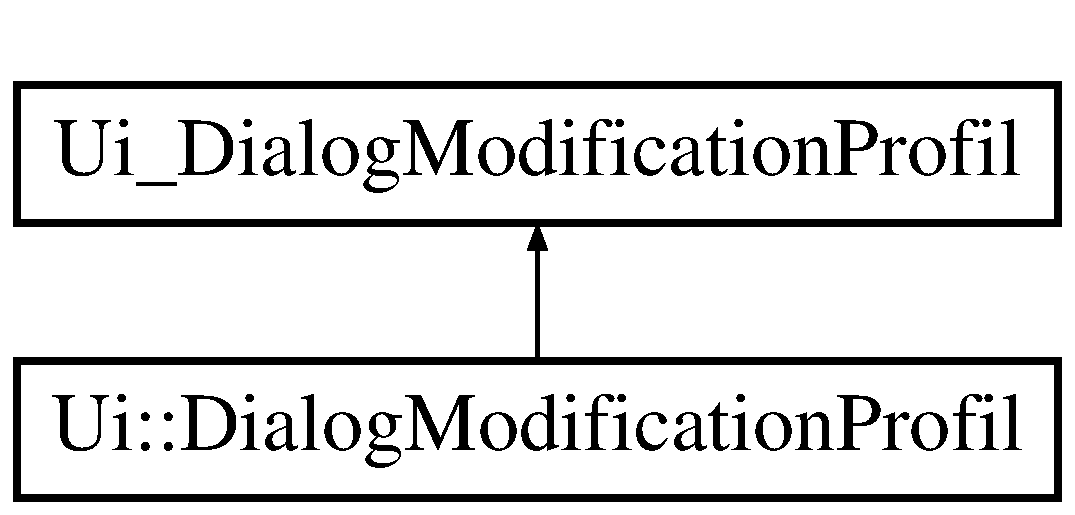
\includegraphics[height=2.000000cm]{class_ui___dialog_modification_profil}
\end{center}
\end{figure}
\subsection*{Fonctions membres publiques}
\begin{DoxyCompactItemize}
\item 
void \hyperlink{class_ui___dialog_modification_profil_a48769dc430bb027d7b0b6df4bcd7146b}{setup\-Ui} (Q\-Dialog $\ast$Dialog\-Modification\-Profil)
\item 
void \hyperlink{class_ui___dialog_modification_profil_aaa740d7d565aabc709ec9b4e5ca46568}{retranslate\-Ui} (Q\-Dialog $\ast$Dialog\-Modification\-Profil)
\end{DoxyCompactItemize}
\subsection*{Attributs publics}
\begin{DoxyCompactItemize}
\item 
Q\-Push\-Button $\ast$ \hyperlink{class_ui___dialog_modification_profil_af20fdf74b0575d4e4a83b3fdd78b773d}{bouton\-Valider}
\item 
Q\-Label $\ast$ \hyperlink{class_ui___dialog_modification_profil_af0cd677e0f1af8ec6649d590537448a0}{label}
\item 
Q\-Line\-Edit $\ast$ \hyperlink{class_ui___dialog_modification_profil_ae95b8fd825c2d092eecd5fdcc83d5213}{nom}
\item 
Q\-Label $\ast$ \hyperlink{class_ui___dialog_modification_profil_abcab2110522286dcc6f1abcfb8df3032}{label\-\_\-3}
\item 
Q\-Line\-Edit $\ast$ \hyperlink{class_ui___dialog_modification_profil_a34af0438ab4d51c5a1cbd3171ca56fbf}{prenom}
\item 
Q\-Label $\ast$ \hyperlink{class_ui___dialog_modification_profil_ae641346202559988ff45516a4ba78e90}{label\-\_\-4}
\item 
Q\-Line\-Edit $\ast$ \hyperlink{class_ui___dialog_modification_profil_a8031c71ba4f8adc3d82bc08d73190f53}{email}
\item 
Q\-Label $\ast$ \hyperlink{class_ui___dialog_modification_profil_ab4a50f6eb1a12c3960b9482bd236a97c}{label\-\_\-5}
\item 
Q\-Line\-Edit $\ast$ \hyperlink{class_ui___dialog_modification_profil_a93b6c690c6707d373fc814a119821546}{code\-\_\-postal}
\item 
Q\-Label $\ast$ \hyperlink{class_ui___dialog_modification_profil_a29db887be1dec97eee38c3a93a765772}{label\-\_\-2}
\item 
Q\-Line\-Edit $\ast$ \hyperlink{class_ui___dialog_modification_profil_a1c6d48ece9604745e80462ef426ac0ea}{ville}
\item 
Q\-Label $\ast$ \hyperlink{class_ui___dialog_modification_profil_a65181d9deaa1b933282b99de2d7240f7}{label\-\_\-6}
\item 
Q\-Label $\ast$ \hyperlink{class_ui___dialog_modification_profil_a04a21015743a0eb5881251fa68c959fa}{label\-\_\-7}
\item 
Q\-Line\-Edit $\ast$ \hyperlink{class_ui___dialog_modification_profil_abd307db23d2f04b3a0e4a596cdbe8656}{adresse}
\end{DoxyCompactItemize}


\subsection{Documentation des fonctions membres}
\hypertarget{class_ui___dialog_modification_profil_aaa740d7d565aabc709ec9b4e5ca46568}{\index{Ui\-\_\-\-Dialog\-Modification\-Profil@{Ui\-\_\-\-Dialog\-Modification\-Profil}!retranslate\-Ui@{retranslate\-Ui}}
\index{retranslate\-Ui@{retranslate\-Ui}!Ui_DialogModificationProfil@{Ui\-\_\-\-Dialog\-Modification\-Profil}}
\subsubsection[{retranslate\-Ui}]{\setlength{\rightskip}{0pt plus 5cm}void Ui\-\_\-\-Dialog\-Modification\-Profil\-::retranslate\-Ui (
\begin{DoxyParamCaption}
\item[{Q\-Dialog $\ast$}]{Dialog\-Modification\-Profil}
\end{DoxyParamCaption}
)\hspace{0.3cm}{\ttfamily [inline]}}}\label{class_ui___dialog_modification_profil_aaa740d7d565aabc709ec9b4e5ca46568}
\hypertarget{class_ui___dialog_modification_profil_a48769dc430bb027d7b0b6df4bcd7146b}{\index{Ui\-\_\-\-Dialog\-Modification\-Profil@{Ui\-\_\-\-Dialog\-Modification\-Profil}!setup\-Ui@{setup\-Ui}}
\index{setup\-Ui@{setup\-Ui}!Ui_DialogModificationProfil@{Ui\-\_\-\-Dialog\-Modification\-Profil}}
\subsubsection[{setup\-Ui}]{\setlength{\rightskip}{0pt plus 5cm}void Ui\-\_\-\-Dialog\-Modification\-Profil\-::setup\-Ui (
\begin{DoxyParamCaption}
\item[{Q\-Dialog $\ast$}]{Dialog\-Modification\-Profil}
\end{DoxyParamCaption}
)\hspace{0.3cm}{\ttfamily [inline]}}}\label{class_ui___dialog_modification_profil_a48769dc430bb027d7b0b6df4bcd7146b}


\subsection{Documentation des données membres}
\hypertarget{class_ui___dialog_modification_profil_abd307db23d2f04b3a0e4a596cdbe8656}{\index{Ui\-\_\-\-Dialog\-Modification\-Profil@{Ui\-\_\-\-Dialog\-Modification\-Profil}!adresse@{adresse}}
\index{adresse@{adresse}!Ui_DialogModificationProfil@{Ui\-\_\-\-Dialog\-Modification\-Profil}}
\subsubsection[{adresse}]{\setlength{\rightskip}{0pt plus 5cm}Q\-Line\-Edit$\ast$ Ui\-\_\-\-Dialog\-Modification\-Profil\-::adresse}}\label{class_ui___dialog_modification_profil_abd307db23d2f04b3a0e4a596cdbe8656}
\hypertarget{class_ui___dialog_modification_profil_af20fdf74b0575d4e4a83b3fdd78b773d}{\index{Ui\-\_\-\-Dialog\-Modification\-Profil@{Ui\-\_\-\-Dialog\-Modification\-Profil}!bouton\-Valider@{bouton\-Valider}}
\index{bouton\-Valider@{bouton\-Valider}!Ui_DialogModificationProfil@{Ui\-\_\-\-Dialog\-Modification\-Profil}}
\subsubsection[{bouton\-Valider}]{\setlength{\rightskip}{0pt plus 5cm}Q\-Push\-Button$\ast$ Ui\-\_\-\-Dialog\-Modification\-Profil\-::bouton\-Valider}}\label{class_ui___dialog_modification_profil_af20fdf74b0575d4e4a83b3fdd78b773d}
\hypertarget{class_ui___dialog_modification_profil_a93b6c690c6707d373fc814a119821546}{\index{Ui\-\_\-\-Dialog\-Modification\-Profil@{Ui\-\_\-\-Dialog\-Modification\-Profil}!code\-\_\-postal@{code\-\_\-postal}}
\index{code\-\_\-postal@{code\-\_\-postal}!Ui_DialogModificationProfil@{Ui\-\_\-\-Dialog\-Modification\-Profil}}
\subsubsection[{code\-\_\-postal}]{\setlength{\rightskip}{0pt plus 5cm}Q\-Line\-Edit$\ast$ Ui\-\_\-\-Dialog\-Modification\-Profil\-::code\-\_\-postal}}\label{class_ui___dialog_modification_profil_a93b6c690c6707d373fc814a119821546}
\hypertarget{class_ui___dialog_modification_profil_a8031c71ba4f8adc3d82bc08d73190f53}{\index{Ui\-\_\-\-Dialog\-Modification\-Profil@{Ui\-\_\-\-Dialog\-Modification\-Profil}!email@{email}}
\index{email@{email}!Ui_DialogModificationProfil@{Ui\-\_\-\-Dialog\-Modification\-Profil}}
\subsubsection[{email}]{\setlength{\rightskip}{0pt plus 5cm}Q\-Line\-Edit$\ast$ Ui\-\_\-\-Dialog\-Modification\-Profil\-::email}}\label{class_ui___dialog_modification_profil_a8031c71ba4f8adc3d82bc08d73190f53}
\hypertarget{class_ui___dialog_modification_profil_af0cd677e0f1af8ec6649d590537448a0}{\index{Ui\-\_\-\-Dialog\-Modification\-Profil@{Ui\-\_\-\-Dialog\-Modification\-Profil}!label@{label}}
\index{label@{label}!Ui_DialogModificationProfil@{Ui\-\_\-\-Dialog\-Modification\-Profil}}
\subsubsection[{label}]{\setlength{\rightskip}{0pt plus 5cm}Q\-Label$\ast$ Ui\-\_\-\-Dialog\-Modification\-Profil\-::label}}\label{class_ui___dialog_modification_profil_af0cd677e0f1af8ec6649d590537448a0}
\hypertarget{class_ui___dialog_modification_profil_a29db887be1dec97eee38c3a93a765772}{\index{Ui\-\_\-\-Dialog\-Modification\-Profil@{Ui\-\_\-\-Dialog\-Modification\-Profil}!label\-\_\-2@{label\-\_\-2}}
\index{label\-\_\-2@{label\-\_\-2}!Ui_DialogModificationProfil@{Ui\-\_\-\-Dialog\-Modification\-Profil}}
\subsubsection[{label\-\_\-2}]{\setlength{\rightskip}{0pt plus 5cm}Q\-Label$\ast$ Ui\-\_\-\-Dialog\-Modification\-Profil\-::label\-\_\-2}}\label{class_ui___dialog_modification_profil_a29db887be1dec97eee38c3a93a765772}
\hypertarget{class_ui___dialog_modification_profil_abcab2110522286dcc6f1abcfb8df3032}{\index{Ui\-\_\-\-Dialog\-Modification\-Profil@{Ui\-\_\-\-Dialog\-Modification\-Profil}!label\-\_\-3@{label\-\_\-3}}
\index{label\-\_\-3@{label\-\_\-3}!Ui_DialogModificationProfil@{Ui\-\_\-\-Dialog\-Modification\-Profil}}
\subsubsection[{label\-\_\-3}]{\setlength{\rightskip}{0pt plus 5cm}Q\-Label$\ast$ Ui\-\_\-\-Dialog\-Modification\-Profil\-::label\-\_\-3}}\label{class_ui___dialog_modification_profil_abcab2110522286dcc6f1abcfb8df3032}
\hypertarget{class_ui___dialog_modification_profil_ae641346202559988ff45516a4ba78e90}{\index{Ui\-\_\-\-Dialog\-Modification\-Profil@{Ui\-\_\-\-Dialog\-Modification\-Profil}!label\-\_\-4@{label\-\_\-4}}
\index{label\-\_\-4@{label\-\_\-4}!Ui_DialogModificationProfil@{Ui\-\_\-\-Dialog\-Modification\-Profil}}
\subsubsection[{label\-\_\-4}]{\setlength{\rightskip}{0pt plus 5cm}Q\-Label$\ast$ Ui\-\_\-\-Dialog\-Modification\-Profil\-::label\-\_\-4}}\label{class_ui___dialog_modification_profil_ae641346202559988ff45516a4ba78e90}
\hypertarget{class_ui___dialog_modification_profil_ab4a50f6eb1a12c3960b9482bd236a97c}{\index{Ui\-\_\-\-Dialog\-Modification\-Profil@{Ui\-\_\-\-Dialog\-Modification\-Profil}!label\-\_\-5@{label\-\_\-5}}
\index{label\-\_\-5@{label\-\_\-5}!Ui_DialogModificationProfil@{Ui\-\_\-\-Dialog\-Modification\-Profil}}
\subsubsection[{label\-\_\-5}]{\setlength{\rightskip}{0pt plus 5cm}Q\-Label$\ast$ Ui\-\_\-\-Dialog\-Modification\-Profil\-::label\-\_\-5}}\label{class_ui___dialog_modification_profil_ab4a50f6eb1a12c3960b9482bd236a97c}
\hypertarget{class_ui___dialog_modification_profil_a65181d9deaa1b933282b99de2d7240f7}{\index{Ui\-\_\-\-Dialog\-Modification\-Profil@{Ui\-\_\-\-Dialog\-Modification\-Profil}!label\-\_\-6@{label\-\_\-6}}
\index{label\-\_\-6@{label\-\_\-6}!Ui_DialogModificationProfil@{Ui\-\_\-\-Dialog\-Modification\-Profil}}
\subsubsection[{label\-\_\-6}]{\setlength{\rightskip}{0pt plus 5cm}Q\-Label$\ast$ Ui\-\_\-\-Dialog\-Modification\-Profil\-::label\-\_\-6}}\label{class_ui___dialog_modification_profil_a65181d9deaa1b933282b99de2d7240f7}
\hypertarget{class_ui___dialog_modification_profil_a04a21015743a0eb5881251fa68c959fa}{\index{Ui\-\_\-\-Dialog\-Modification\-Profil@{Ui\-\_\-\-Dialog\-Modification\-Profil}!label\-\_\-7@{label\-\_\-7}}
\index{label\-\_\-7@{label\-\_\-7}!Ui_DialogModificationProfil@{Ui\-\_\-\-Dialog\-Modification\-Profil}}
\subsubsection[{label\-\_\-7}]{\setlength{\rightskip}{0pt plus 5cm}Q\-Label$\ast$ Ui\-\_\-\-Dialog\-Modification\-Profil\-::label\-\_\-7}}\label{class_ui___dialog_modification_profil_a04a21015743a0eb5881251fa68c959fa}
\hypertarget{class_ui___dialog_modification_profil_ae95b8fd825c2d092eecd5fdcc83d5213}{\index{Ui\-\_\-\-Dialog\-Modification\-Profil@{Ui\-\_\-\-Dialog\-Modification\-Profil}!nom@{nom}}
\index{nom@{nom}!Ui_DialogModificationProfil@{Ui\-\_\-\-Dialog\-Modification\-Profil}}
\subsubsection[{nom}]{\setlength{\rightskip}{0pt plus 5cm}Q\-Line\-Edit$\ast$ Ui\-\_\-\-Dialog\-Modification\-Profil\-::nom}}\label{class_ui___dialog_modification_profil_ae95b8fd825c2d092eecd5fdcc83d5213}
\hypertarget{class_ui___dialog_modification_profil_a34af0438ab4d51c5a1cbd3171ca56fbf}{\index{Ui\-\_\-\-Dialog\-Modification\-Profil@{Ui\-\_\-\-Dialog\-Modification\-Profil}!prenom@{prenom}}
\index{prenom@{prenom}!Ui_DialogModificationProfil@{Ui\-\_\-\-Dialog\-Modification\-Profil}}
\subsubsection[{prenom}]{\setlength{\rightskip}{0pt plus 5cm}Q\-Line\-Edit$\ast$ Ui\-\_\-\-Dialog\-Modification\-Profil\-::prenom}}\label{class_ui___dialog_modification_profil_a34af0438ab4d51c5a1cbd3171ca56fbf}
\hypertarget{class_ui___dialog_modification_profil_a1c6d48ece9604745e80462ef426ac0ea}{\index{Ui\-\_\-\-Dialog\-Modification\-Profil@{Ui\-\_\-\-Dialog\-Modification\-Profil}!ville@{ville}}
\index{ville@{ville}!Ui_DialogModificationProfil@{Ui\-\_\-\-Dialog\-Modification\-Profil}}
\subsubsection[{ville}]{\setlength{\rightskip}{0pt plus 5cm}Q\-Line\-Edit$\ast$ Ui\-\_\-\-Dialog\-Modification\-Profil\-::ville}}\label{class_ui___dialog_modification_profil_a1c6d48ece9604745e80462ef426ac0ea}


La documentation de cette classe a été générée à partir du fichier suivant \-:\begin{DoxyCompactItemize}
\item 
/home/magalie/\-Bureau/\-S5/\-C\-P\-O\-O\-A/\-Projet/\-E-\/\-Marche-\//iterations/iteration2/\-E\-Marche/\hyperlink{ui___dialog_modification_profil_8h}{ui\-\_\-\-Dialog\-Modification\-Profil.\-h}\end{DoxyCompactItemize}

\hypertarget{class_vue}{\section{Référence de la classe Vue}
\label{class_vue}\index{Vue@{Vue}}
}


The \hyperlink{class_vue}{Vue} class -\/ Permet la mise à jour des vues.  




{\ttfamily \#include $<$Vue.\-h$>$}

Graphe d'héritage de Vue\-:\begin{figure}[H]
\begin{center}
\leavevmode
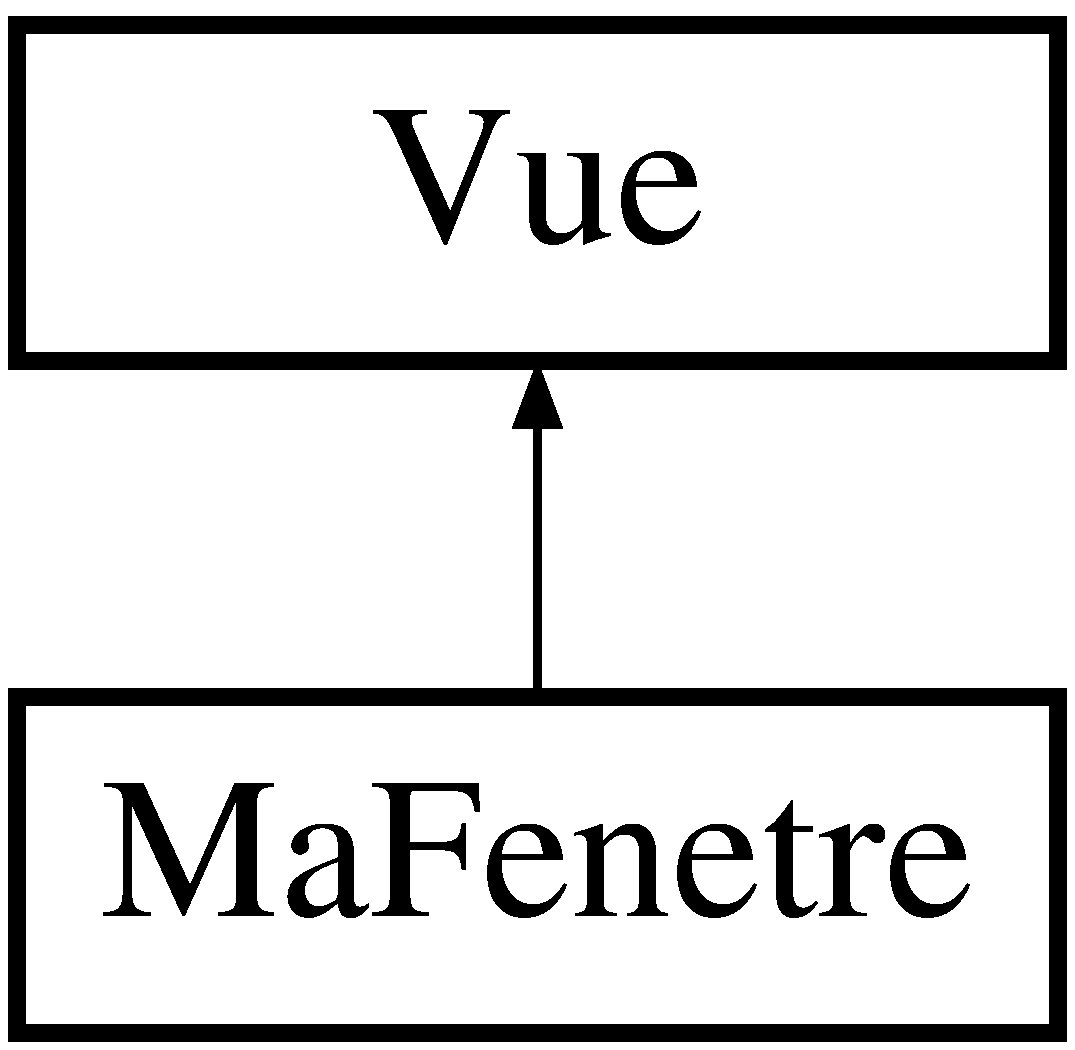
\includegraphics[height=2.000000cm]{class_vue}
\end{center}
\end{figure}
\subsection*{Fonctions membres publiques}
\begin{DoxyCompactItemize}
\item 
virtual \hyperlink{class_vue_a527643b4a1f794f495c464209d0318a2}{$\sim$\-Vue} ()
\item 
virtual void \hyperlink{class_vue_a49c501f530bbe66414c415c438ec0695}{update} ()=0
\begin{DoxyCompactList}\small\item\em update -\/ Mise à jour \end{DoxyCompactList}\end{DoxyCompactItemize}


\subsection{Description détaillée}
The \hyperlink{class_vue}{Vue} class -\/ Permet la mise à jour des vues. 

\subsection{Documentation des constructeurs et destructeur}
\hypertarget{class_vue_a527643b4a1f794f495c464209d0318a2}{\index{Vue@{Vue}!$\sim$\-Vue@{$\sim$\-Vue}}
\index{$\sim$\-Vue@{$\sim$\-Vue}!Vue@{Vue}}
\subsubsection[{$\sim$\-Vue}]{\setlength{\rightskip}{0pt plus 5cm}virtual Vue\-::$\sim$\-Vue (
\begin{DoxyParamCaption}
{}
\end{DoxyParamCaption}
)\hspace{0.3cm}{\ttfamily [inline]}, {\ttfamily [virtual]}}}\label{class_vue_a527643b4a1f794f495c464209d0318a2}


\subsection{Documentation des fonctions membres}
\hypertarget{class_vue_a49c501f530bbe66414c415c438ec0695}{\index{Vue@{Vue}!update@{update}}
\index{update@{update}!Vue@{Vue}}
\subsubsection[{update}]{\setlength{\rightskip}{0pt plus 5cm}virtual void Vue\-::update (
\begin{DoxyParamCaption}
{}
\end{DoxyParamCaption}
)\hspace{0.3cm}{\ttfamily [pure virtual]}}}\label{class_vue_a49c501f530bbe66414c415c438ec0695}


update -\/ Mise à jour 



Implémenté dans \hyperlink{class_ma_fenetre_a342da912af9b611d47229fd190d68522}{Ma\-Fenetre}.



La documentation de cette classe a été générée à partir du fichier suivant \-:\begin{DoxyCompactItemize}
\item 
/home/magalie/\-Bureau/\-S5/\-C\-P\-O\-O\-A/\-Projet/\-E-\/\-Marche-\//iterations/iteration4/\-E\-Marche/\hyperlink{_vue_8h}{Vue.\-h}\end{DoxyCompactItemize}

%--- End generated contents ---

% Index
\newpage
\phantomsection
\addcontentsline{toc}{chapter}{Index}
\printindex

\end{document}
